\documentclass[titlepage]{article}

\usepackage{graphicx} % for embedding pictures
\usepackage{wrapfig} % for use with figures
\usepackage{tikz} % for doing flow charts and stuff directly inside of latex
\usepackage{framed} % if you want a frame around a figure
\usepackage[hidelinks]{hyperref} % allows embedding links
\usepackage[T1]{fontenc} % fixes weird font size/encoding issues
\usepackage[utf8]{inputenc} % ensures input is UTF-8
\usepackage{listings} % used to format code
\usepackage{algorithm} % used with the below package to format psuedo code
\usepackage[noend]{algpseudocode}
\usepackage{mathtools} % used for all the mathematical notation
\usepackage{etaremune} % enumerate backwards for OSI model
\usepackage{booktabs} % used for tables and making them look slick as
\usepackage{placeins} % used to ensure everything stays inside where it is 
% defined, i.e. subsections jumping above figures etc.
\usepackage[nopostdot]{glossaries} % guess what. It manages glossaries
\setacronymstyle{long-short}
\makenoidxglossaries{}

% load the glossary
\loadglsentries{glossary}

% define some colours for code
\definecolor{dkgreen}{rgb}{0,0.6,0}
\definecolor{gray}{rgb}{0.5,0.5,0.5}
\definecolor{mauve}{rgb}{0.58,0,0.82}

% code formatting options
\lstset{%
  frame=tb,
  showstringspaces=false,
  columns=flexible,
  basicstyle={\small\ttfamily},
  numbers=left,
  numberstyle=\tiny\color{gray},
  keywordstyle=\color{blue},
  commentstyle=\color{dkgreen},
  stringstyle=\color{mauve},
  breaklines=true,
  breakatwhitespace=true
}


% diagramming options
\usetikzlibrary{shapes.geometric, arrows, arrows.meta, positioning}

% flow chart styles
\tikzstyle{startstop} = [
  rectangle,
  rounded corners,
  minimum width=3cm,
  minimum height=1cm,
  text centered,
  draw=black,
  inner sep=0,
  fill=red!30
]
\tikzstyle{io} = [
  trapezium,
  trapezium left angle=60,
  trapezium right angle=120,
  minimum width=3cm,
  minimum height=1cm,
  text centered,
  text width=3cm,
  inner sep=0,
  draw=black,
  trapezium stretches=true,
  fill=blue!30
]
\tikzstyle{process} = [
  rectangle,
  minimum width=3cm,
  minimum height=1cm,
  text centered,
  text width=3cm,
  inner sep=0,
  draw=black,
  fill=orange!30
]
\tikzstyle{decision} = [
  diamond,
  minimum width=3cm,
  minimum height=1cm,
  text centered,
  draw=black,
  aspect=2,
  inner sep=0,
  fill=green!30
]
\tikzstyle{arrow} = [
  thick,
  ->,
  =stealth
]

% data flow diagram styles
\tikzstyle{function} = [
  circle,
  inner sep=0pt,
  draw=black,
  minimum width=1cm,
  minimum height=1cm,
  text width=2cm,
  text centered,
  fill=red!20
]
\tikzstyle{inputoutput} = [
  rectangle,
  draw=black,
  minimum width=3cm,
  minimum height=1cm,
  text width=3cm,
  text centered,
  fill=blue!20
]
\tikzstyle{datastore} = [
  rectangle,
  inner sep=0pt,
  minimum height=1cm,
  minimum width=3cm,
  text width=3cm,
  text centered,
  fill=green!20
]
\tikzstyle{method} = [
  rectangle,
  draw=black,
  fill=gray!30,
  minimum width=2cm,
  minimum height=0.5cm,
  text centered
]

% ladder diagram lines
\tikzstyle{connecting arrow} = [-{Latex[length=2mm, width=3mm, green]}]
\tikzstyle{closing arrow} = [-{Latex[length=2mm, width=3mm, red]}]
\tikzstyle{normal arrow} = [-{Latex[length=2mm, width=3mm, blue]}]
\tikzstyle{with slope} = [above, midway, sloped]


% forces [sub]sections to contain everything that is defined before the next one
\let\Oldsection\section{}
\renewcommand{\section}{\FloatBarrier\Oldsection}

\let\Oldsubsection\subsection{}
\renewcommand{\subsection}{\FloatBarrier\Oldsubsection}

\let\Oldsubsubsection\subsubsection{}
\renewcommand{\subsubsection}{\FloatBarrier\Oldsubsubsection}


% title
\author{Sam Leonard}
\title{A Level Computer Science Non-Examined Assessment (NEA)}
\date{} % this forces no date to be shown

\begin{document}

\maketitle

\tableofcontents

\section{Analysis}

\subsection{Identification and Background to the Problem}

The problem I am trying to solve with my project is how to look at devices on a network from a 
``\gls{bbox}'' perspective and gain information about what \glspl{service} are running etc. Services 
are programs which their entire purpose is to provide a \textit{\gls{service}} to other programs, 
for example a server hosting a website would be running a \gls{service} whose purpose is to send the 
webpage to people who try to connect to the website. \\ 
There are many steps in-between a device turning on to interacting with the internet.

\begin{enumerate}
  \item{load networking \glspl{driver}}
  \item{Starting \gls{dhcp} \gls{daemon}}
  \item{Broadcasting \gls{dhcp} request for an \gls{ipaddr}}
  \item{Get assigned an \gls{ipaddr}}
\end{enumerate}

There are many more steps than I have listed above but these are the most important ones. Starting 
from a linux computer being switched on the first step is that the \gls{kernel} needs to load the 
networking \glspl{driver}. The \gls{kernel} is the basis for the operating system, it is what 
interacts with the hardware in the most fundamental way. \glspl{driver} are small bits of code which 
the \gls{kernel} can load in order to interact with certain hardware modules such as the \gls{nic} 
which is essential for interfacing with the network, hence the name.

Next once the \gls{kernel} has loaded the required \glspl{driver} and the system has booted the 
networking `\glspl{daemon}' must be started. In linux a \gls{daemon} is a program that runs all the 
time in the background to serve a specific purpose or utility. For example when I start my laptop 
the following \glspl{daemon} start \gls{upow} (power management), \gls{sysd} (manages the creation 
of all processes), \gls{dbus} (manages inter-process communication), iwd (manages my WiFi 
connections) and finally \gls{dhcpcd} which manages all interactions with the network around 
\gls{dhcp}.

Once the \glspl{daemon} are all started the \gls{dhcp} client can now take issue commands to the 
daemon for it to carry out. The \gls{dhcp} client is simply a daemon that runs in the background to 
carry out any interactions between the current machine and the \gls{dhcp} server. The \gls{dhcp} 
server is normally the WiFi router or network switch for the local network and it manages a list of 
which computer has which \gls{ipaddr} and negotiates with new computers trying to join a network to 
get them a free \gls{ipaddr}. The \gls{dhcp} client starts the \gls{dhcp} address negotiation with 
the server by sending a discover message with the address 255.255.255.255 which is the IP limited 
broadcast address which means that whatever is listening at the other end will forward this 
\gls{pkt} on to everyone on the \gls{subnet}. When the \gls{dhcp} \gls{server} (normally the router, 
sometimes a separate machine) on the subnet receives this message it reserves a free \gls{ipaddr} 
for that client and then responds with a \gls{dhcp} offer which contains the address the 
\gls{server} is offering, the length of time the address is valid for and the \gls{subnet} mask of 
the network. The client must then respond with a \gls{dhcp} request message to request the offered 
address, this is in case of multiple DHCP servers offering addresses. Finally the \gls{dhcp} server 
responds with a \gls{dhcp} acknowledge message showing that it has received the request. 
Figure~\ref{dhcp_negotiate} shows a \gls{pkt} capture from my laptop where I turned WiFi off, 
started wireshark listening and plugged in an Ethernet cable, I have it showing only the \gls{dhcp} 
\glspl{pkt} so that it is clear to see the entire \gls{dhcp} negotiation including the 
255.255.255.255 limited broadcast destination address and the 0.0.0.0 unassigned address in the 
source column. I mention using wireshark to do packet capturing above without explaining what either 
packet capturing or wireshark are so I will do that here. Packets I define below and wireshark is 
simply a tool which intercepts all the network communications on a single computer and records them 
to a file as well as displaying them to the user as well as performing some analysis and dissecting 
each of the protocols used. This means that I can record the \gls{dhcp} negotiation shown below and 
show it to you using wireshark to get all the information out of the packets being sent over the 
wire.
\begin{figure}[H]

  \begin{framed}

  \centering
  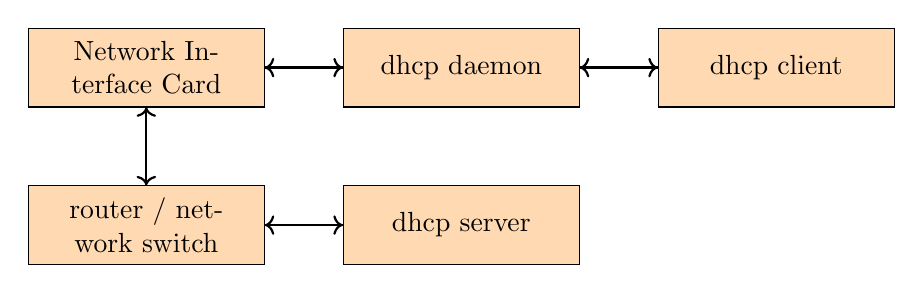
\begin{tikzpicture}[node distance=2cm]

    \node (nic) [process] {Network Interface Card};
    \node (router) [process, below of=nic] {router / network switch};
    \node (daemon) [process, right of=nic, xshift=2cm] {\gls{dhcp} daemon};
    \node (client) [process, right of=daemon, xshift=2cm] {\gls{dhcp} client};
    \node (server) [process, right of=router, xshift=2cm] {\gls{dhcp} server};

    \draw [arrow] (nic) -- (router);
    \draw [arrow] (router) -- (nic);
    \draw [arrow] (server) -- (router);
    \draw [arrow] (router) -- (server);
    \draw [arrow] (nic) -- (daemon);
    \draw [arrow] (daemon) -- (nic);
    \draw [arrow] (client) -- (daemon);
    \draw [arrow] (daemon) -- (client);

  \end{tikzpicture}

  \end{framed}

  \caption{%
    A block diagram showing the relationship between
    different elements of a \gls{dhcp} negotiation.
  }\label{dhcpdiagram}
\end{figure}

\begin{figure}[H]
  \centering
  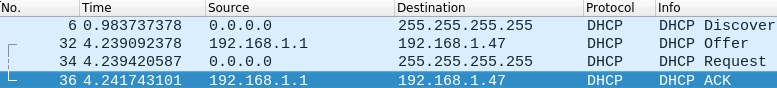
\includegraphics[width=\textwidth]{screenshots/dhcp_negotiation.png}
  \caption{\gls{dhcp} address negotiation}\label{dhcp_negotiate}
\end{figure}

All computer networking is encapsulated in the \gls{osi} which has 7 layers:

\begin{etaremune}
  \item{Application: \gls{api}s, \gls{http}, \gls{ftp} among others.}
  \item{Presentation: encryption/decryption, encoding/decoding, decompression etc\ldots}
  \item{Session: Managing sessions, \gls{php} session IDs etc\ldots}
  \item{Transport: TCP and UDP among others.}
  \item{Network: ICMP and IP among others.}
  \item{Data Link: MAC addressing, Ethernet protocol etc\ldots}
  \item{Physical: The physical Ethernet cabling/\gls{nic}.}
\end{etaremune}

\begin{figure}[H]
  \centering
  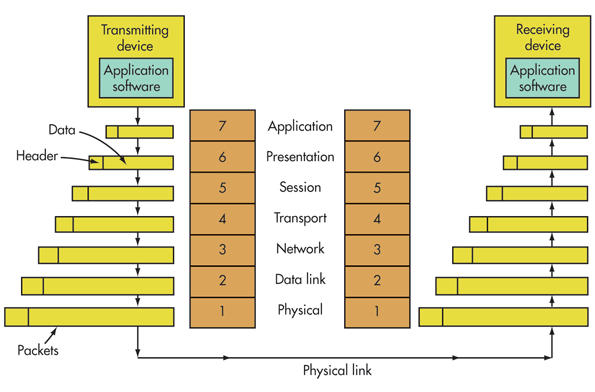
\includegraphics[width=\textwidth]{screenshots/osi_model.png}
  \caption{%
    OSI model diagram, source: https://www.electronicdesign.com
  }\label{osi_model}
\end{figure}
Each of these layers is essential to the running of the internet but a single communication might 
not include all of the layers. These communications are all based on the most fundamental part of 
the internet: the \gls{pkt}. Packets are sequences of ones and zeros sent between computers which 
are used to transfer data as well as to control how networks function. They consist of different 
layers of information each specifying where the \gls{pkt} where should go next at a different level 
along with fundamentally the data/instructions contained in the innermost layer. When \glspl{pkt} 
are sent between computers a certain number of layers are stripped off by each computer so that it 
knows where to send the \gls{pkt} next at which point it will add all the layers back again, this 
time with the instructions needed to go from the current computer to the next one on its route. Each 
of these layers actually consists of a number of fields at the start called a \gls{header} some 
layers also append a footer to the end of the packet. The actual data being transferred in the 
packet can be quite literally anything, \gls{http} transfers websites so \gls{html} files and images 
etc\ldots. In particular there are two pieces of information stored in headers which together define 
the final destination of the packet: the \gls{ipaddr} and the \gls{port} number. The \gls{ipaddr} 
defines the destination machine and the \gls{port} number defines which ``port'' on the remote 
machine the packet should be sent to. Ports are essential entrances to a computer, for example if a 
computer was a hotel the \gls{ipaddr} would be the address and location of the hotel and the 
\gls{port} number would be the room inside the hotel. There are 65535 \glspl{port} and 0 is a 
special reserved port. Both \gls{tcp} and \gls{udp} use \glspl{port}, \gls{tcp} \glspl{port} are 
mainly used for transferring data where reliability is a concern, as \gls{tcp} has built in checks 
for packet loss whereas \gls{udp} does not and as such is used for purposes where speed is more 
important and missing some data is inconsequential, such as video streaming and playing games. 

I'm going to use the example of getting a very simple static HTML page with an image inside. The 
code for the page is shown in listing~\ref{examplepage}. In figure~\ref{basicwebpage} you can see 
how the page renders. However far more interestingly is how the browser retrieved the page, in 
figure~\ref{getrequest} you can see the full sequence of \glspl{pkt} that were exchanged for the 
browser to get the resources it needed to render the page. I am hosting the page using Python3's 
http.server module which is super convenient and just makes the current directory open on port 8000 
from there I can just navigate to /example.html and it will render the page. Breaking 
figure~\ref{getrequest} down \gls{pkt} one shows the browser receiving the request from the user to 
display \verb|http://192.168.1.47:8000/example.html| and attempting to connect to 192.168.1.47 on 
port 8000. Packets two and three show the negotiation of this request through to the full connection 
being made. The browser now makes an \gls{http} GET request for the page example.html over the 
established TCP connection as shown in \gls{pkt} 4. The server then acknowledges the request and 
sends a \gls{pkt} with the PSH flag set as shown in \glspl{pkt} 6 and 7. The PSH flag is a request 
to the browser to say that it is OK to received the buffered data, i.e.\ example.html. The browser 
then sends back an acknowledgement and the server sends the page as shown in \glspl{pkt} 7 and 8. 
Finally the browser sends a final acknowledgement of having received the page before initiating a 
graceful session teardown by sending a FIN ACK \gls{pkt} which indicates the end of a session. Once 
the server responds to the FIN ACK with it's own the browser sends a final acknowledgement. This 
then repeats itself when the browser parses the HTML and realises theres an image which it needs to 
get from the server as well, except the image is a larger file and so takes a few more PSH 
\glspl{pkt}. In figures~\ref{getrequestladder} and~\ref{ladder} you can see a set of ladder diagrams
which show the entire transaction symbolically. I have also colour coded figure~\ref{ladder} with
green arrow heads to the initial handshakes, blue for the HTTP protocol transactions and red for
the TCP connection teardown packets.

This shows clearly the interaction between each of the different layers in the OSI model,
the browser at level 7: Application rendering the webpage. Level 6: Presentation is skipped as
we have no files which need to be served compressed because they are so large. Level 5: Session
is shown by the TCP session negotiation and graceful teardown of the TCP session. Level 4: Transport
is shown when the image and webpage are transferred from the server to the browser. Level 3/2/1
are shown in figure~\ref{deconstructed} where you can see the IP layer information along with
Ethernet II and finally frame 4 which is the bytes that went down the wire.

\begin{figure}[H]
  \centering
  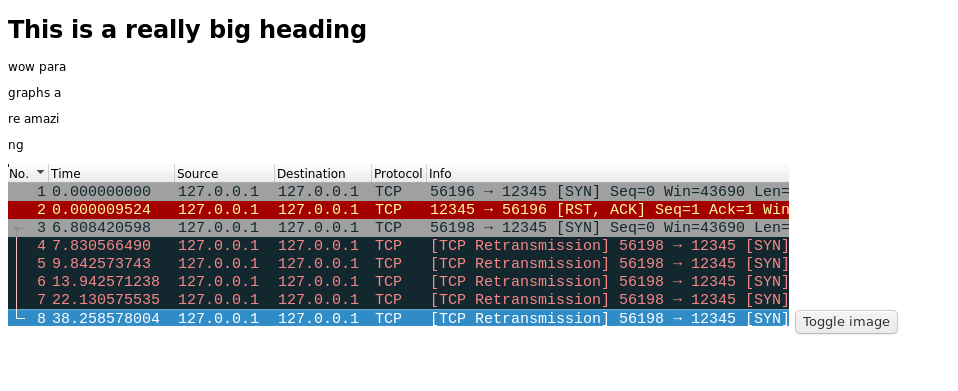
\includegraphics[width=\textwidth]{screenshots/basic_webpage.png}
  \caption{%
    A basic static \gls{html} webpage.
  }\label{basicwebpage}
\end{figure}

\begin{figure}[H]
  \centering
  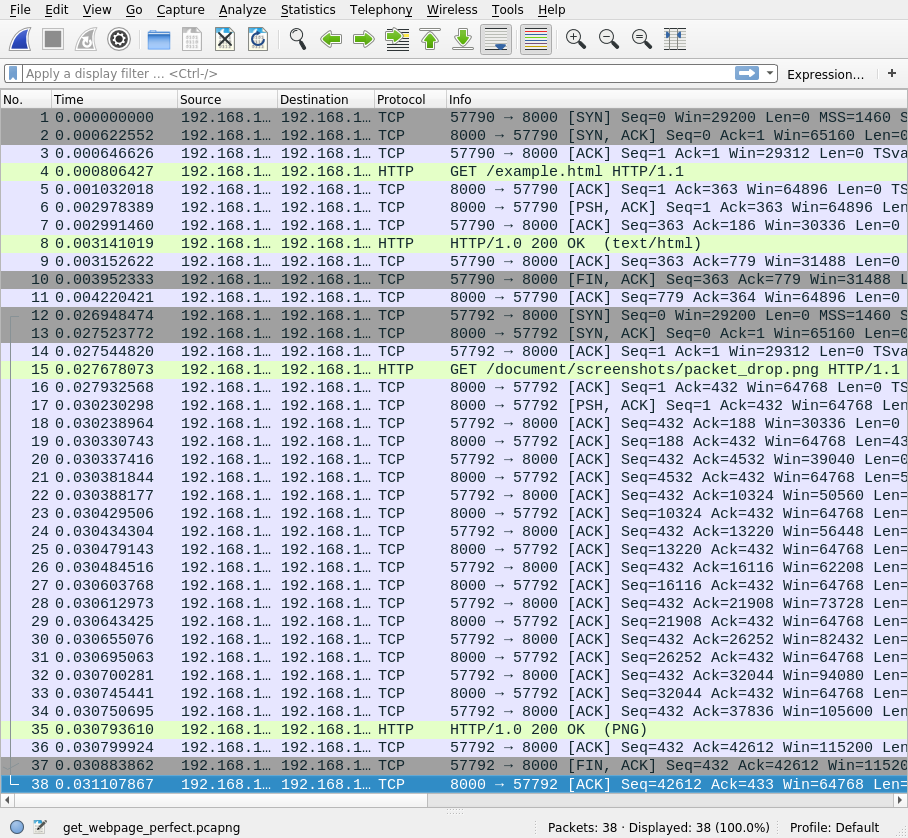
\includegraphics[width=\textwidth]{screenshots/website_get.png}
  \caption{%
    A full chain of \glspl{pkt} that shows retrieving a basic webpage
    from the server.
  }\label{getrequest}
\end{figure}

\begin{figure}[H]
  \centering
  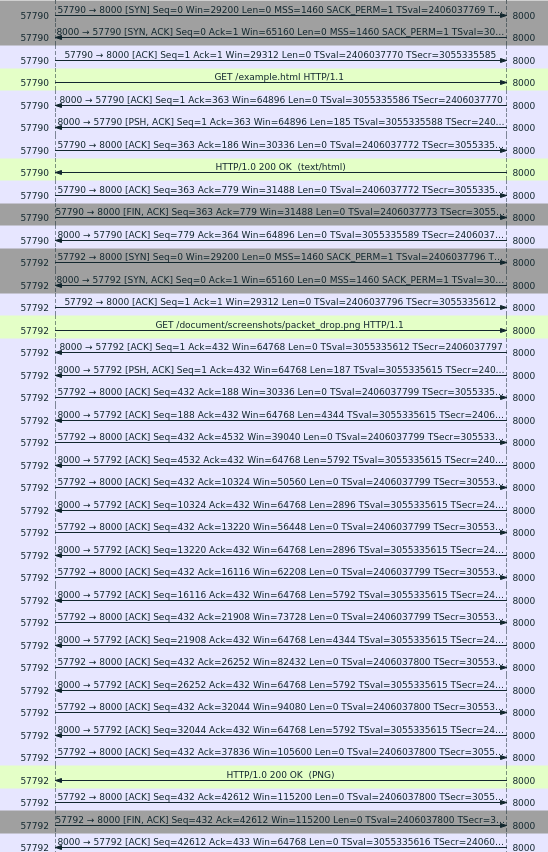
\includegraphics[width=\textwidth]{screenshots/website_get_ladder.png}
  \caption{%
    Ladder diagram of figure~\ref{getrequest}.
  }\label{getrequestladder}
\end{figure}

\begin{figure}[H]
  \centering
  \begin{framed}
  
\begin{tikzpicture}
    \node[rectangle,minimum width=.8\textwidth,minimum height=.8\textheight] (ladder) {};
      \draw[black,very thick] (ladder.north west) -- (ladder.south west);
      \draw[black,very thick] (ladder.north east) -- (ladder.south east);
    \node[above of=ladder, xshift=-4.5cm,yshift=7cm] (local 0) {local machine};
    \node[above of=ladder, xshift=4.5cm, yshift=7cm] (web 0) {webserver};
    \foreach \i [count=\j from 0]in {1,...,14}{
      \node [below=0.85cm of local \j] (local \i) {};
      \node [below=0.85cm of web \j] (web \i) {};
    }

    \draw[connecting arrow] (local 0) -- node[with slope] {SYN} (web 1);
    \draw[connecting arrow]   (web 1) -- node[with slope] {SYN, ACK} (local 2);
    \draw[connecting arrow] (local 2) -- node[with slope] {ACK} (web 3);
    \draw[normal arrow]     (local 3) -- node[with slope] {HTTP GET /example.html} (web 4);
    \draw[normal arrow]       (web 4) -- node[with slope] {HTTP 200 OK} (local 5);
    \draw[closing arrow]    (local 5) -- node[with slope] {FIN, ACK} (web 6);
    \draw[closing arrow]      (web 6) -- node[with slope] {ACK} (local 7);
    \draw[connecting arrow] (local 7) -- node[with slope] {SYN} (web 8);
    \draw[connecting arrow]   (web 8) -- node[with slope] {SYN, ACK} (local 9);
    \draw[connecting arrow] (local 9) -- node[with slope] {ACK} (web 10);
    \draw[normal arrow]    (local 10) -- node[with slope] {HTTP GET /document/screenshots/packet\_drop.png} (web 11);
    \draw[normal arrow]      (web 11) -- node[with slope] {HTTP 200 OK} (local 12);
    \draw[closing arrow]   (local 12) -- node[with slope] {FIN, ACK} (web 13);
    \draw[closing arrow]     (web 13) -- node[with slope] {ACK} (local 14);

  \end{tikzpicture}
  \end{framed}
  \caption{%
    A simplified ladder diagram showing the transaction in figure~\ref{getrequest}
  }\label{ladder}
\end{figure}

\begin{figure}[H]
  \centering
  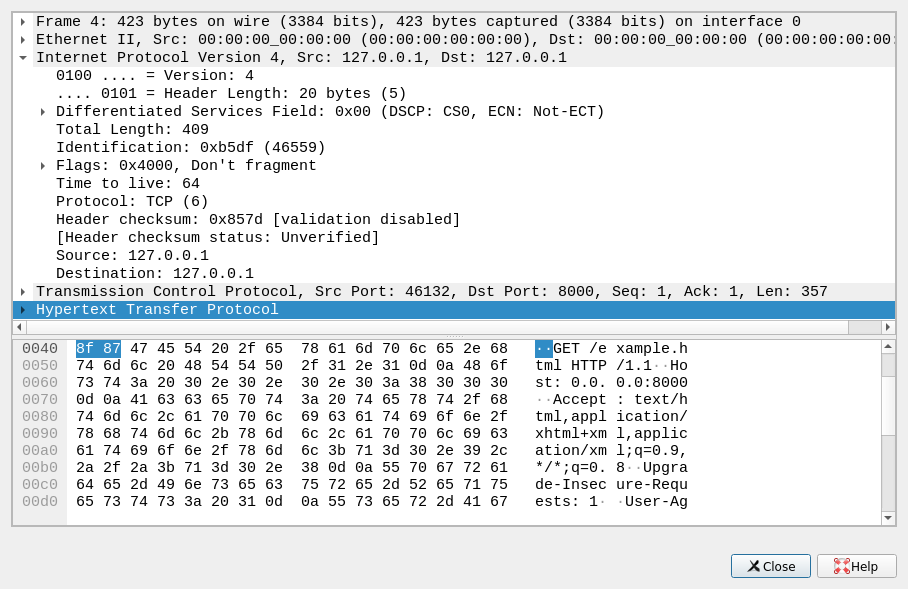
\includegraphics[width=\textwidth]{screenshots/deconstructed_packet.png}
  \caption{%
    A look inside a TCP \gls{pkt}.
  }\label{deconstructed}
\end{figure}

\lstset{language=HTML}
\lstinputlisting[caption={example.html}, label={examplepage}]{../example.html}

\subsection{Analysis of problem}

The problem with looking at a network from the outside is that the purpose of the network is to 
allow communication inside of the network, thus very little is exposed externally. This presents a 
challenge as we want to know what is on the network as well as what each of them is running which is 
not always possible due to the limited information that \glspl{service} will reveal about 
themselves. Firewalls also play large part in making scanning networks difficult as sometimes they 
simply drop \glspl{pkt} instead of sending a \gls{tcp} RST \gls{pkt} (reset connection \gls{pkt}). 
When firewalls drop \glspl{pkt} it becomes exponentially more difficult as you don't know whether 
your \gls{pkt} was corrupted or lost in transit or if it was just dropped. \\\\ To demonstrate this 
I will show three things:

\begin{enumerate}
  \item{A successful connection over \gls{tcp}.}
  \item{An attempted connection to a closed port.}
  \item{An attempted connection with a firewall rule to drop packets.}
\end{enumerate}

Firstly A successful \gls{tcp} connection. For a \gls{tcp} connection to be established there is a 
three way handshake between the communicating machines. Firstly the machine trying to establish the 
connection sends a \gls{tcp} SYN packet to the other machine, this packet holds a dual purpose, to 
ask for a connection and if it is accepted to SYNchronise the sequence numbers being used to detect 
whether packets have been lost in transport. The receiving machine then replies with a \gls{tcp} SYN 
ACK which confirms the starting sequence number with the SYN part and ACKnowledges the connection 
request. The sending machine then acknowledges this by sending a final \gls{tcp} ACK packet back. 
This connection initialisation is shown in figure~\ref{data_transfer} by packets one, two and three. 
Data transfer can then commence by sending a \gls{tcp} packet with the PSH and ACK flags set along 
with the data in the data portion of the packet, this is shown in figure~\ref{data} where wireshark 
allows us to take a look inside the packet to see the data being sent in the packet along with the 
PSH and ACK flags being set. The code I used to generate these is shown in figures~\ref{sender} 
and~\ref{receiver}. Breaking the code down in figure~\ref{receiver} you can see me initialising a 
socket object then I bind it to localhost (127.0.0.1) port 12345 localhost is just an address which 
allows connections between programs running on the same computer as connections are looped back onto 
the current machine, hence its alternative name: the loopback address. I then tell it to listen for 
incoming connections, the one just means how many connections to keep as a backlog. I then accept 
the connection from the program in figure~\ref{sender}, line 3. I then tell the program to listen 
for up to 1024 bytes in the data part of any TCP packets sent. The program in figure~\ref{sender} 
then sends some data which we then see printed to the screen in figure~\ref{receiver}, both programs 
then close the connection.

\begin{figure}[H]
  \centering
  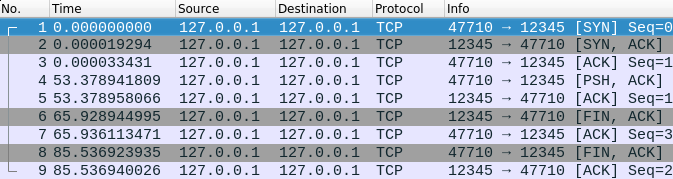
\includegraphics[width=\textwidth]{screenshots/data_transfer.png}
  \caption{%
    Packets starting a TCP session, transferring some data then ending it.
  }\label{data_transfer}
\end{figure}

\begin{figure}[H]
  \centering
  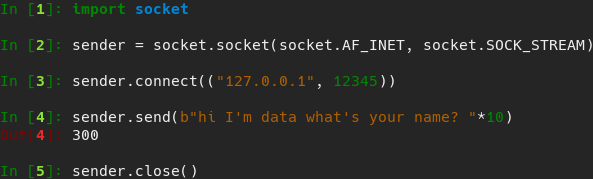
\includegraphics[width=\textwidth]{screenshots/sender.png}
  \caption{%
    Transferring some basic text data over a TCP connection.
  }\label{sender}
\end{figure}

\begin{figure}[H]
  \centering
  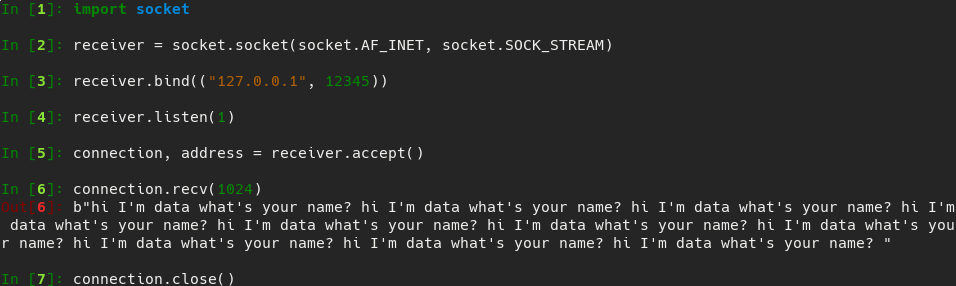
\includegraphics[width=\textwidth]{screenshots/receiver.png}
  \caption{%
    Receiving some basic text data over a TCP connection.
  }\label{receiver}
\end{figure}

\begin{figure}[H]
  \centering
  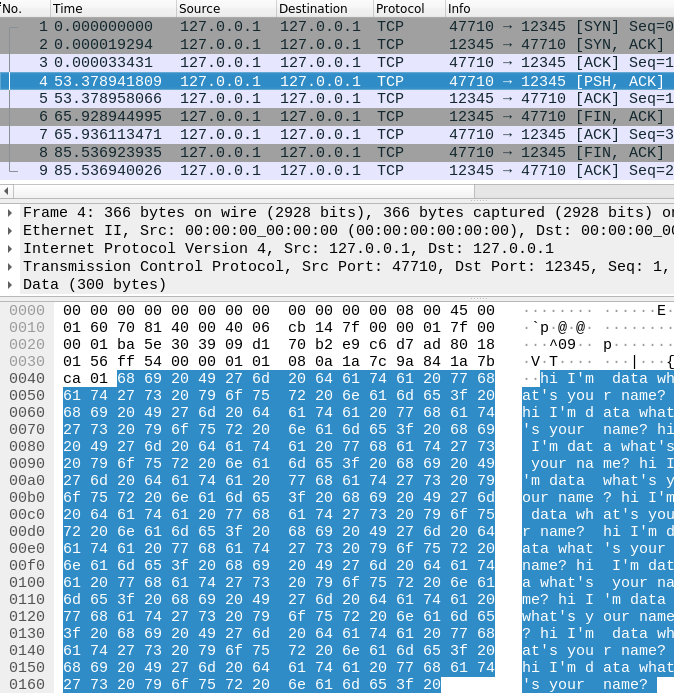
\includegraphics[width=\textwidth]{screenshots/data.png}
  \caption{%
    Highlighted packet carrying the data being transferred in figure~\ref{sender}.
  }\label{data}
\end{figure}

Next an attempted connection to a closed port. In figure~\ref{firewall} packet one you can see
the same \gls{tcp} SYN packet as we saw in the attempted connection to an open port, as you
would expect. The difference comes in the next packet with the \gls{tcp} RST flag being sent
back. This flag means to reset the connection, or if the connection is not yet established
as in this case it means that the port is closed, hence why the packet is highlighted red
in figure~\ref{firewall}. The code used to generate this is shown in figure~\ref{firewall_code}
line two shows the initialisation of a socket object. In line 3 the program tries to connect
to port 12345 on localhost again, except this time we get a connection refused error back
this shows us that the remote host sent a \gls{tcp} RST packet back, which is reflected in
figure~\ref{firewall}.

Finally I will show a connection where the firewall is configured to drop the packet. However first 
I will explain a bit about firewalls and how they work. Firewalls are essentially the gatekeepers of 
the internet they decide whether a packet gets to pass or whether they shall not pass. Firewalls 
work by a set of rules which decide what happens to it. A rule might be that it is coming from a 
certain \gls{ipaddr} or has a certain destination port. The actions taken after the packet has had 
it's fate decided by the rules can be one of the following three (on iptables on linux): ACCEPT, 
DROP and RETURN, accept does exactly what you think it would an lets the packet through, drop quite 
literally just drops the packet and sends no reply whatsoever, return is more complicated and has no 
effect on how port scanning is done and as such we will ignore it. A common set of rules for 
something like a webserver would be to DROP all incoming packets and then allow exceptions for 
certain ports i.e.\ port 80 for \gls{http} or 443 for \gls{https}. I will be using a linux utility 
called iptables for implementing all firewall rules on my system for demonstration purposes. Packet 
number three in figure~\ref{firewall} shows the connection request from line 4 
of~\ref{firewall_code} except that I have enabled a firewall rule to drop all \glspl{pkt} from the 
address 127.0.0.1, using the iptables command as so: \verb$iptables -I INPUT -s 127.0.0.1 -j DROP$. 
This command reads as for all \glspl{pkt} arriving (\verb|-I INPUT|) with source address 127.0.0.1 
(\verb|-s 127.0.0.1|) drop them sending no response (\verb|-j DROP|). With this firewall rule in 
place you can see in figure~\ref{firewall} \gls{pkt} 3 receives no response and as such Python 
assumes that the \gls{pkt} just got lost and as such tries to send the \gls{pkt} again repeatedly, 
this continued for more than 30 seconds before a stopped it as shown by the time column in 
figure~\ref{firewall} and the final \verb|KeyboardInterrupt| in figure~\ref{firewall_code}. The 
amount of time that a system will wait still trying to reconnect depends on the OS and a other 
factors but the minimum time is 100 seconds as specified by RFC 1122, on most systems it will be 
between 13 and 30 minutes according the linux manual page on \gls{tcp}.

\begin{verbatim}
man 7 tcp:
tcp_retries2 (integer; default: 15; since Linux 2.2)
  The maximum number of times a TCP packet is retransmitted in
  established state before giving up. The default value is 15,
  which corresponds to a duration of approximately between 13 to 30
  minutes, depending on the retransmission timeout. The RFC 1122
  specified minimum limit of 100 seconds is typically deemed too short.
\end{verbatim}

\begin{figure}[H]
  \centering
  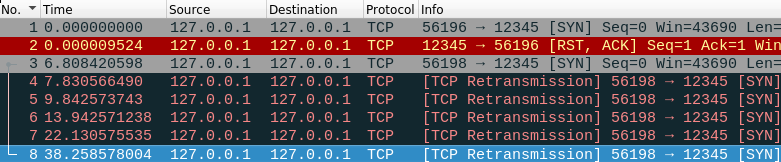
\includegraphics[width=\textwidth]{screenshots/packet_drop.png}
  \caption{%
    Attempted connection to a closed port with and without firewall rule to drop \glspl{pkt}.
  }\label{firewall}
\end{figure}

\begin{figure}[H]
  \centering
  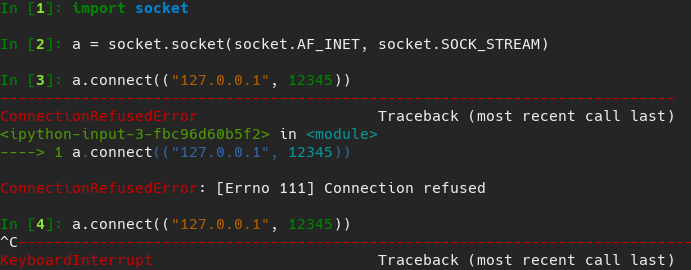
\includegraphics[width=\textwidth]{screenshots/packet_drop_code.png}
  \caption{%
    The code used to produce firewall \gls{pkt} dropping example in figure~\ref{firewall}
  }\label{firewall_code}
\end{figure}

Having explained firewalls, how they affect port scanning and other things above I will now explain 
what I am actually trying to achieve with my project and how I am going to do it. I am trying to 
make a tool similar to nmap which will be able to detect the state (as in whether the port is 
open/closed or filtered etc) of ports on remote machines, detect which hosts are up on a subnet and 
finally I want to be able to try to detect what services are listening behind any of the ports. I am 
going to be writing in Python version 3.7.2 as it is the latest stable release of Python 3 and has 
many features which are not in even fairly recent versions such as 3.5, the biggest one of these 
being fstrings which are where I can put a single a `f' before a string and then any formatting 
options I put inside using curly braces are expanded and formatted accordingly. This allows for a 
clear and consistent string formatting syntax which I will use extensively. I will be using Python 
in particular as a language because it is very readable and has extensive low level bindings to C 
networking functions with the socket module allowing me to write code quickly which is easily 
understandable and has a clear purpose and at the same time be able to use low level networking 
functions and even changing the behaviour at this low level with \verb|socket.setsockopt|. As well 
as this the socket module allows me to open sockets that communicate using many different protocols 
such as \gls{tcp}, \gls{udp} and \gls{icmp} just to name a few. These features combine to make 
Python a great language for writing networking software with a high level of abstraction. In regards 
to the OSI model my code will sit with the user interface at level 7 specifying what to do at a high 
level then the actual scanning takes place at levels 3, 4 and 5 with host detection being at level 
3. Port scanning will be taking place At level 4 for \gls{tcp} SYN scanning and \gls{udp} scanning. 
Whereas \verb|connect()| scanning and version detection will sit at level 5. Finally I will look at 
what is actually handling all of the networking on my machine. My machine runs linux and as such all 
networking is handled by system calls to the linux kernel. For example the \verb|socket.connect| 
method is just a call to the underlying linux kernel's connect syscall but presenting a kinder call 
signature to the user as the Python socket library does some processing before the syscall is made. 

\subsection{Success Criteria}

\begin{enumerate}

  \item{%
    Probe another computer's networking from a \gls{bbox} perspective.
  }
  \item{%
    Send \gls{icmp} ECHO requests to determine whether a machine is active
    or not.
  }
  \item{%
    Translate \gls{cidr} specified subnets into a list of domains.
  }
  \item{%
    Detect whether a TCP port is open (can be connected to).
  }
  \item{%
    Detect whether a TCP port is closed (will refuse connections).
  }
  \item{%
    Detect whether a TCP port is filtered (a firewall is
    preventing or monitoring access).
  }
  \item{%
    Detect whether a UDP port is open (can be connected to).
  }
  \item{%
    Detect whether a UDP port is closed (will refuse connections).
  }
  \item{%
    Detect whether a UDP port is filtered (a firewall is
    preventing or monitoring access).
  }
  \item{%
    Detect the operating system of another machine on the network
    solely from sending packets to the machine and interpreting the responses.
  }
  \item{%
    Detect what service is listening behind a port.
  }
  \item{%
    Detect the version of the service running behind a port.
  }

\end{enumerate}

\subsection{Description of current system or existing solutions}

Nmap is currently the most popular tool for doing\gls{port}scanning and host enumeration.
It supports the scanning types for determining information about remote hosts.

\begin{itemize}
  \item{\gls{tcp}:\ SYN}
  \item{\gls{tcp}:\ \verb|Connect()|}
  \item{\gls{tcp}:\ ACK}
  \item{\gls{tcp}:\ Window}
  \item{\gls{tcp}:\ Maimon}
  \item{\gls{tcp}:\ Null}
  \item{\gls{tcp}:\ FIN}
  \item{\gls{tcp}:\ Xmas}
  \item{\gls{udp}}
  \item{Zombie host/idle}
  \item{\gls{sctp}:\ INIT}
  \item{\gls{sctp}:\ COOKIE-ECHO}
  \item{IP protocol scan}
  \item{\gls{ftp}:\ bounce scan}
\end{itemize}

As well as supporting a vast array of scanning types it also can do \gls{service} version detection 
and operating system detection via custom probes. Nmap also has script scanning which allows the 
user to write a script specifying exactly how they want to scan e.g.\ to circumvent \gls{port 
knocking} (where \glspl{pkt} must be sent to a sequence of \glspl{port} in order before access to 
the final\gls{port}is allowed). It also supports a plethora of options to avoid firewalls or 
\gls{ids} such as sending \glspl{pkt} with spoofed \glspl{csum}/source addresses and sending decoy 
probes. Nmap can do many more things than I have listed above as is illustrated quite clearly by the
fact there is an entire working on using nmap 
(\href{https://nmap.org/book/}{https://nmap.org/book/}). The following is an example nmap scan
which I did on my home network: \verb|nmap -sC -sV -oA networkscan 192.168.1.0/24|. Breaking
it down this means to enable script scanning \verb|-sc|, enable version detection \verb|-sV|
and then output all results in all the common formats: XML, nmap and greppable, using the
base name \verb|networkscan| which produces three files: \verb|networkscan.(nmap,gnmap,xml)|.
Before I go into what each file contains I will explain some terminology, greppable is anything
which can be easily searched with the linux \verb|grep| which stands for Globally search a Regular
Expression and Print, which basically means look in files for lines that contain a certain word
or pattern, for example finding all lines with the word ``hi'' in them in the file ``document''
\verb|grep hi document|. Onto the files: \verb|networkscan.nmap| contains what would usually
be printed by nmap while the scan is being run, it looks like this:
\begin{verbatim}
# Nmap 7.70 scan initiated Wed Apr 10 19:36:18 2019 as:
    nmap -sC -sV -oA /home/tritoke/thing 192.168.1.0/24
Nmap scan report for router.asus.com (192.168.1.1)
Host is up (1.0s latency).
Not shown: 995 closed ports
PORT     STATE SERVICE    VERSION
53/tcp   open  domain     (generic dns response: NOTIMP)
| fingerprint-strings: 
|   DNSVersionBindReqTCP: 
|     version
|_    bind
80/tcp   open  http       ASUS WRT http admin
|_http-server-header: httpd/2.0
|_http-title: Site doesn't have a title (text/html).
515/tcp  open  printer
8443/tcp open  ssl/http   ASUS WRT http admin
|_http-server-header: httpd/2.0
|_http-title: Site doesn't have a title (text/html).
| ssl-cert: Subject: commonName=192.168.1.1/countryName=US
| Not valid before: 2018-05-05T05:05:17
|_Not valid after:  2028-05-05T05:05:17
9100/tcp open  jetdirect?
1 service unrecognized despite returning data. If you know the service/version,
please submit the following fingerprint at
https://nmap.org/cgi-bin/submit.cgi?new-service :
SF-Port53-TCP:V=7.70%I=7%D=4/10%Time=5CAE3DC5%P=x86_64-pc-linux-gnu%r(DNSV
SF:ersionBindReqTCP,20,"\0\x1e\0\x06\x85\x85\0\x01\0\0\0\0\0\0\x07version\
SF:x04bind\0\0\x10\0\x03")%r(DNSStatusRequestTCP,E,"\0\x0c\0\0\x90\x04\0\0
SF:\0\0\0\0\0\0");
Service Info: CPE: cpe:/o:asus:wrt_firmware
\end{verbatim}
Above is just the report for one such device in the report as the full thing is over 200 lines lone.
In it you can see information such as which ports are open and what services are running behind them
as this is my router you can see port 8443 which nmap has recognised to be hosting the ASUS web
admin from which you can configure the route. Then after than some other associated information
extracted from the server. Most of this extra information is from the \verb|-sC| flag which is
script scanning and allows advanced interaction with running services specifically to gain more
information by providing specialised probing per protocol. We can also see at the end an
unrecognised service which nmap shows us the data it returned and asks us to submit a new service
report at a given URL if we recognise the service. This system of submitting fingerprints of
services is how nmap is so good at recognising services: it has a lot of data to look at and learn
from in regards to service fingerprinting.

Next \verb|networkscan.gnmap|:
\begin{verbatim}
# Nmap 7.70 scan initiated Wed Apr 10 19:36:18 2019 as:
    nmap -sC -sV -oA /home/tritoke/networkscan 192.168.1.0/24
Host: 192.168.1.1 (router.asus.com) Status: Up
Host: 192.168.1.1 (router.asus.com) Ports: 53/open/tcp//domain//
      (generic dns response: NOTIMP)/, 80/open/tcp//http//ASUS WRT http admin/,
      515/open/tcp//printer///, 8443/open/tcp//ssl|http//ASUS WRT http admin/,
      9100/open/tcp//jetdirect?///  Ignored State: closed (995)
Host: 192.168.1.8 (android-25a97e36c2e74456)  Status: Up
Host: 192.168.1.8 (android-25a97e36c2e74456)  Ports: 5060/filtered/tcp//sip///
      Ignored State: closed (999)
\end{verbatim}
Again this is not all of the file as it is very large. As you can see above all of the information 
is on a single line for each type of scan, this is useful if you want to scan a large number of 
hosts and just want to know which hosts are up you can do \verb|grep 'Status: Up' networkscan.gnmap|
which outputs this:
\begin{verbatim}
$ grep 'Status: Up' networkscan.gnmap
Host: 192.168.1.1 (router.asus.com) Status: Up
Host: 192.168.1.8 (android-25a97e36c2e74456) Status: Up
Host: 192.168.1.10 (diskstation) Status: Up
Host: 192.168.1.88 () Status: Up
Host: 192.168.1.88 () Status: Up
Host: 192.168.1.117 () Status: Up
Host: 192.168.1.159 (groot) Status: Up
Host: 192.168.1.159 (groot) Status: Up
Host: 192.168.1.176 (ET0021B7C01F2E) Status: Up
\end{verbatim}
Showing you clearly the hosts which are online and then their host names. Other ways to use this
output format would be to find out which ports are open on only one machine, or which hosts have a
webserver running on them or a vulnerable version of a mail server etc. In general it is useful for
when you want to filter results.

Finally we have \gls{xml} format:
\lstset{language=xml}
\begin{lstlisting}
<?xml version="1.0" encoding="UTF-8"?>
<!DOCTYPE nmaprun>
<?xml-stylesheet href="file:///usr/bin/../share/nmap/nmap.xsl" type="text/xsl"?>
<!-- Nmap 7.70 scan initiated Wed Apr 10 19:36:18 2019 as: nmap -sC -sV -oA /home/tritoke/thing 192.168.1.0/24 -->
<nmaprun scanner="nmap" args="nmap -sC -sV -oA /home/tritoke/thing 192.168.1.0/24" start="1554921378" startstr="Wed Apr 10 19:36:18 2019" version="7.70" xmloutputversion="1.04">
<verbose level="0"/>
<debugging level="0"/>
<host starttime="1554921379" endtime="1554923187"><status state="up" reason="syn-ack" reason_ttl="0"/>
<address addr="192.168.1.1" addrtype="ipv4"/>
<hostnames>
<hostname name="router.asus.com" type="PTR"/>
</hostnames>
<ports><extraports state="closed" count="995">
<extrareasons reason="conn-refused" count="995"/>
</extraports>
<port protocol="tcp" portid="53"><state state="open" reason="syn-ack" reason_ttl="0"/><service name="domain" extrainfo="generic dns response: NOTIMP" servicefp="SF-Port53-TCP:V=7.70%I=7%D=4/10%Time=5CAE3DC5%P=x86_64
-pc-linux-gnu%r(DNSVersionBindReqTCP,20,&quot;\0\x1e\0\x06\x85\x85\0
\x01\0\0\0\0\0\0\x07version\x04bind\0\0\x10\0\x03&quot;)%r
(DNSStatusRequestTCP,E,&quot;\0\x0c\0\0\x90\x04\0\0\0\0\0\0\0\0&quot;);" method="probed" conf="10"/><script id="fingerprint-strings" output="&#xa;  DNSVersionBindReqTCP: &#xa;    version&#xa;    bind"><elem key="DNSVersionBindReqTCP">&#xa;    version&#xa;    bind</elem>
</script></port>
\end{lstlisting}
It is verbose in the extreme contains the reason why each port has the state it does as well as a
vast amount of other data that the other scans didn't include as well as this it is not very human
readable meaning that this format is more likely available because it is easier for other programs
to parse than the other formats. As well as this the verbosity can be good if you really need to
dive into why a port was marked as closed etc or the exact bytes that a service replied with.

In terms of where nmap lives in the software stack is that it is an application at level 7 when the
user interacts with it but it uses several libraries which interact at level 2 which it uses to get
the raw headers of the packets being sent and thus gain information from them.

\begin{figure}[H]

  \begin{framed}

  \centering
  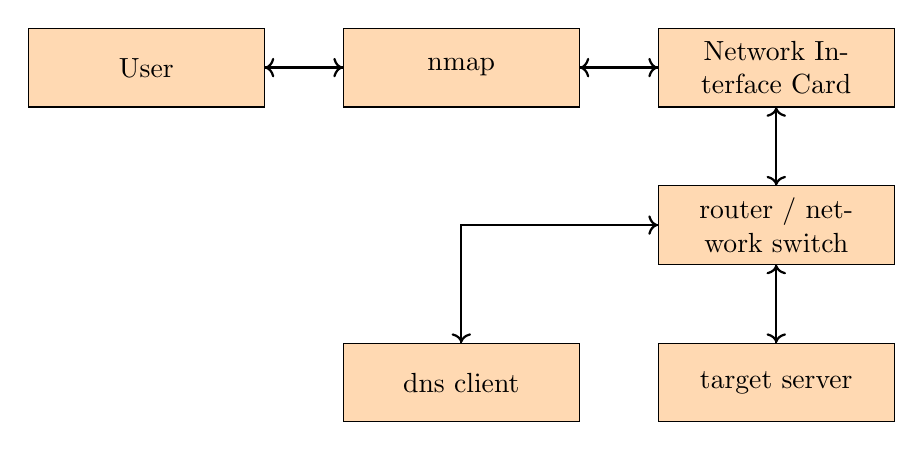
\begin{tikzpicture}[node distance=2cm]

    \node (user) [process] {User};
    \node (nmap) [process, right of=user, xshift=2cm] {nmap};
    \node (nic) [process, right of=nmap, xshift=2cm] {Network Interface Card};
    \node (router) [process, below of=nic] {router / network switch};
    \node (target) [process, below of=router] {target server};
    \node (dnsserver) [process, left of=target, xshift=-2cm] {\gls{dns} client};

    \draw [arrow] (nic) -- (router);
    \draw [arrow] (router) -- (nic);
    \draw [arrow] (target) -- (router);
    \draw [arrow] (router) -- (target);
    \draw [arrow] (dnsserver) |- (router);
    \draw [arrow] (router) -| (dnsserver);
    \draw [arrow] (nic) -- (nmap);
    \draw [arrow] (nmap) -- (nic);
    \draw [arrow] (user) -- (nmap);
    \draw [arrow] (nmap) -- (user);

  \end{tikzpicture}

  \end{framed}

  \caption{%
    A block diagram showing how nmap sits in the software stack.
  }\label{nmapblock}

\end{figure}

\begin{figure}[H]
  \hspace{2cm}
  \begin{framed}

  \centering
  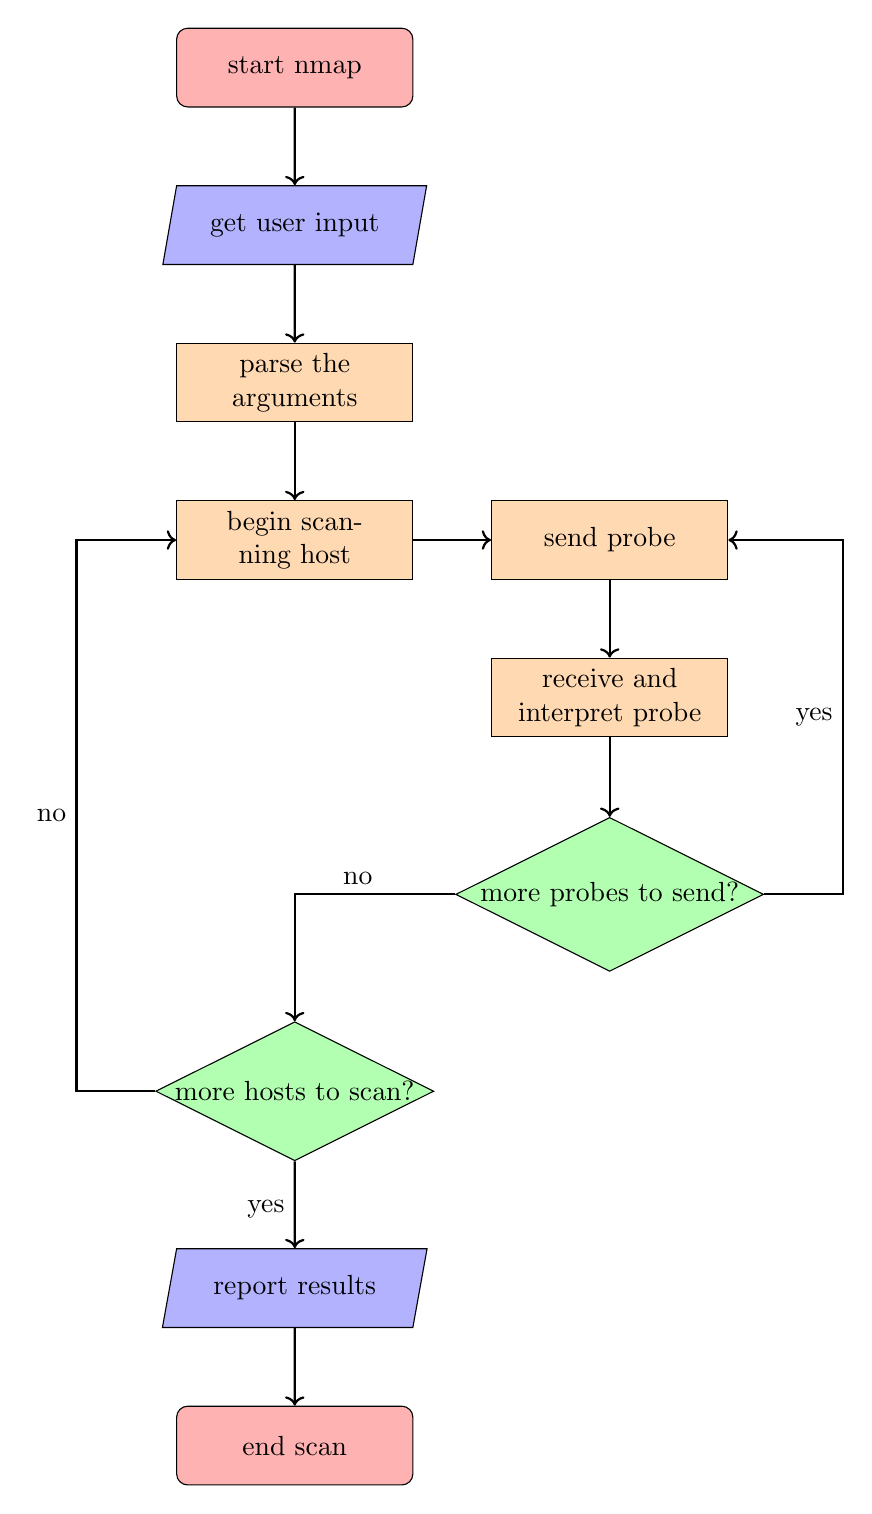
\begin{tikzpicture}[node distance=2cm]

    \node (start) [startstop] {start nmap};
    \node (get) [io, below of=start] {get user input};
    \node (arguments) [process, below of=get] {parse the arguments};
    \node (host) [process, below of=arguments] {begin scanning host};
    \node (probe) [process, right of=host, xshift=2cm] {send probe};
    \node (response) [process, below of=probe] {receive and interpret probe};
    \node (probes) [decision, below of=response, yshift=-0.5cm] {more probes to send?};
    \node (hosts) [decision, left of=probes, below of=probes, xshift=-2cm, yshift=-0.5cm] {more hosts to scan?};
    \node (report) [io, below of=hosts, yshift=-0.5cm] {report results};
    \node (end) [startstop, below of=report] {end scan};

    \draw [arrow] (start) -- (get);
    \draw [arrow] (get) -- (arguments);
    \draw [arrow] (arguments) -- (host);
    \draw [arrow] (host) -- (probe);
    \draw [arrow] (probe) -- (response);
    \draw [arrow] (response) -- (probes);
    \draw [arrow] (probes) -- ([xshift=1cm]probes.east) node[anchor=east,yshift=2.25cm] {yes} |- (probe.east);
    \draw [arrow] (probes) -| node[anchor=south,xshift=0.8cm] {no} (hosts);
    \draw [arrow] (hosts) -- ([xshift=-1cm]hosts.west) node[anchor=east,yshift=3.5cm] {no} |- (host);
    \draw [arrow] (hosts) node[anchor=east,yshift=-1.5cm] {yes} -- (report);
    \draw [arrow] (report) -- (end);

  \end{tikzpicture}

  \end{framed}

  \caption{%
    A flow chart showing how nmap does scanning.
  }\label{nmapflow}

\end{figure}

\subsection{Prospective Users}

The prospective users of this system would be system administrators, penetration testers or network
engineers. In my case my prospective users would be my school's system administrators and it would 
allow them to see an outsiders perspective on for example the \gls{server} running the school's 
website page or to see if any of the programs on the \glspl{server} were leaking information
through \glspl{banner} etc. (most \glspl{service} send a \gls{banner} with information like what
protocol version they use and other information) 

\subsection{Data Dictionary}

So while my program is running it will need to store many different things in memory:
\begin{itemize}
  \item{the list of hosts to scan}
  \item{the list of ports to scan on each host}
  \item{the state of each port we are scanning on each host}
  \item{the packet received by the listening socket (temporarily before processing)}
  \item{various counters and positional indicators are almost inevitable}
  \item{the probes to be used for version detection}
\end{itemize}
So I am going to try to estimate the amount of RAM my program will use based on scanning a 
\gls{cidr} specified subnet of 192.168.1.0/24, and the most common ports 1000 ports of each machine
I will not consider version detection as I am unsure of how I will implement it currently.
To measure the size of object in python we can use the \verb|getsizeof| function provided by the
\verb|sys| module, I also have a file called `hosts' which contains the addresses specified by
192.168.1.0/24 and a file `ping\_bytes' which contains 4 captured packets from the ping command
which I captured during an early exploratory testing phase.
\lstset{language=python}
\begin{lstlisting}[label=testingsize,caption=some testing I did on the size of python objects]
>>> with open("hosts", "r") as f:
...     hosts = f.read().splitlines()
... 
>>> import sys
>>> sys.getsizeof(hosts)
2216
>>> ports = list(range(1000))
>>> sys.getsizeof(ports)
9112
>>> len(hosts)*sys.getsizeof(ports) / 2**10  # 2*10 is one kibibyte
2278.0
>>> sys.getsizeof(True)
28
>>> len(hosts)*(sys.getsizeof(True)) / 2**10
7.0
>>> pings[0]
'45 00 00 54 0f 82 40 00 40 01 2d 25 7f 00 00 01 7f 00 00 01 08 00 41 c5 02 4f 00 01 cd ef 0f 5c de 9b 0d 00 08 09 0a 0b 0c 0d 0e 0f 10 11 12 13 14 15 16 17 18 19 1a 1b 1c 1d 1e 1f 20 21 22 23 24 25 26 27 28 29 2a 2b 2c 2d 2e 2f 30 31 32 33 34 35 36 37'
>>> from binascii import unhexlify
>>> ping = unhexlify(pings[0].replace(" ", ""))  # turn the string of numbers into a bytes object
>>> sys.getsizeof(ping)
117
>>> len(hosts)*sys.getsizeof(ping) / 2**10
29.25
>>> 2278.0 + 7.0 + 29.25 + 2.22
2316.47
\end{lstlisting}
As shown in Listing~\ref{testingsize} we can see that by far the most space intensive item stored
by our program will be the port numbers for each host, making up just less that ninety six percent
of the total space used by the mock data I created. However overall 2.3 mebibytes is not a huge
amount of data by any means.

\begin{center}
  \begin{tabular}{p{3cm} l r r}
    \toprule
    Holding    & Data type   & Space used /Kib & Percentage of total \\
    \midrule
    ports      & List[int]   & 2278            & 98.34 \\
    hosts      & List[str]   & 2.22            & 0.1   \\
    port state & List[bool]  & 7               & 0.3   \\
    packets    & List[bytes] & 29.25           & 1.26  \\
    \bottomrule
  \end{tabular}
\end{center}

\subsection{Data Flow Diagram}

In my application there will be three way information flow: 
\begin{enumerate}
  \item{sending packets (data) out from my application}
  \item{receiving packets back from the targets}
  \item{how my program sends data around between functions}
\end{enumerate}

\begin{figure}[H]
  \centering
  \begin{framed}
  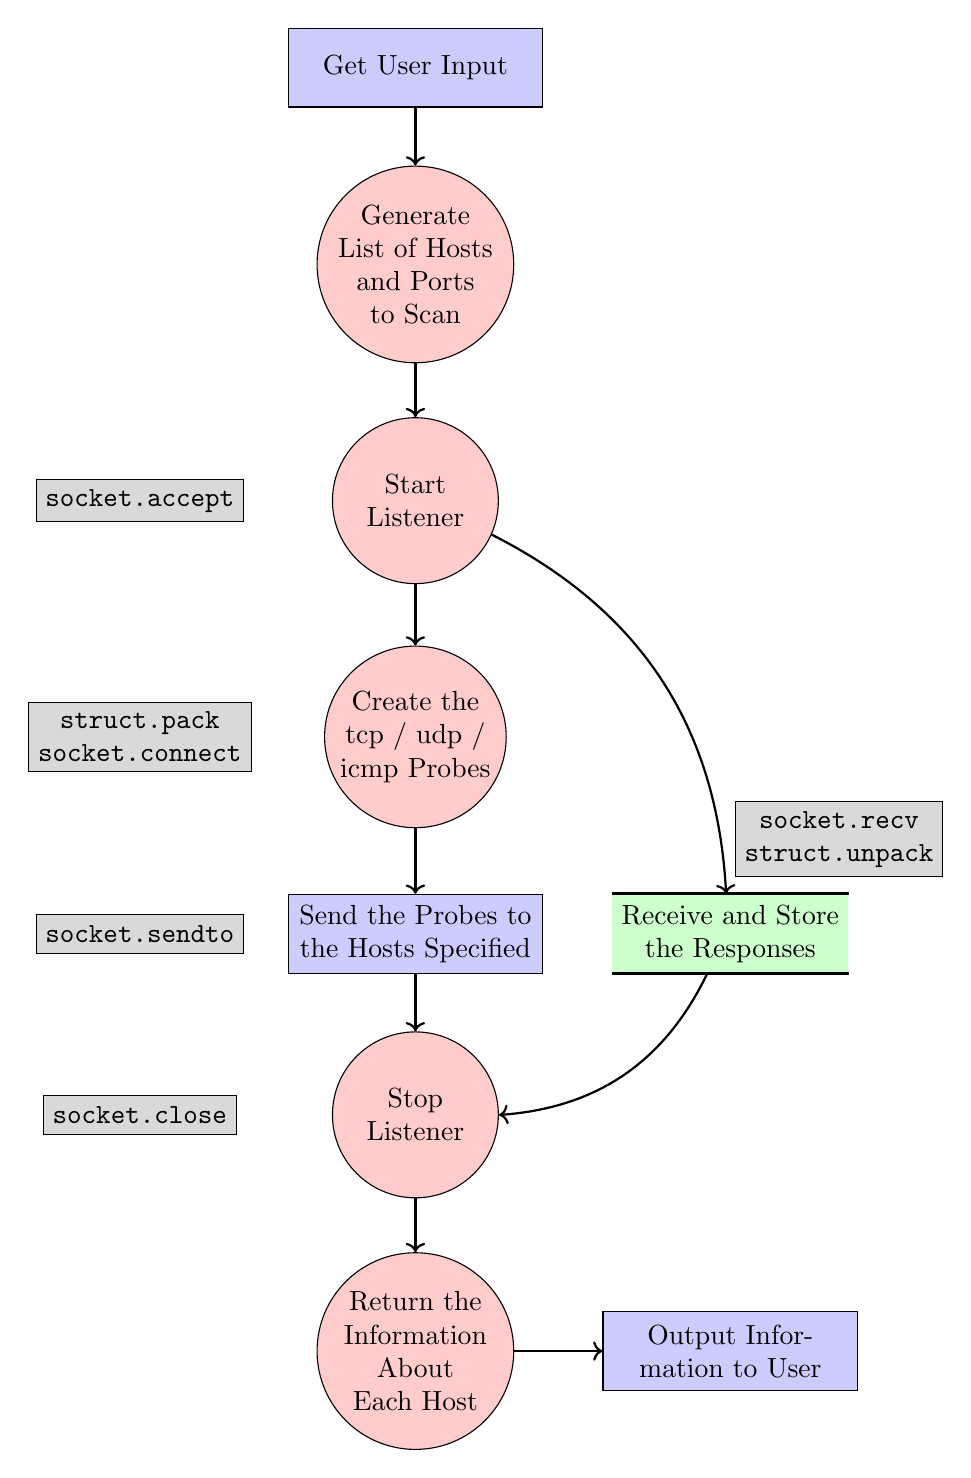
\begin{tikzpicture}[node distance=2cm]
    % \node [function] (no) {hi};
    % \node [inputoutput, below of=no] (beans) {for you};
    \node [inputoutput] (input) {Get User Input};
    \node [function, below of=input, yshift=-0.5cm] (hosts) {Generate List of Hosts and Ports to Scan};
    \node [function, below of=hosts, yshift=-1cm] (listen) {Start Listener};
    \node [function, below of=listen, yshift=-1cm] (create) {Create the \gls{tcp} / \gls{udp} / \gls{icmp} Probes};
    \node [inputoutput, below of=create, yshift=-0.5cm] (send) {Send the Probes to the Hosts Specified};
    \node [function, below of=send,yshift=-0.3cm] (stop) {Stop Listener};
    \node [datastore, right of=stop, xshift=2cm, yshift=2.3cm] (responses) {Receive and Store the Responses};
      \draw [black,very thick] (responses.north west) -- (responses.north east);
      \draw [black,very thick] (responses.south west) -- (responses.south east);
    \node [function, below of=stop, yshift=-1cm] (return) {Return the Information About Each Host};
    \node [inputoutput, right of=return, xshift=2cm] (finish) {Output Information to User};
    \node [method,left of=listen, xshift=-1.5cm] {\verb|socket.accept|};
    \node [method,left of=create, xshift=-1.5cm, text width=2.6cm] {\verb|struct.pack| \verb|socket.connect|};
    \node [method,left of=send, xshift=-1.5cm] {\verb|socket.sendto|};
    \node [method,left of=stop, xshift=-1.5cm] {\verb|socket.close|};
    \node [method,right of=responses,yshift=1.2cm,xshift=-0.62cm,text width=2.4cm] {\verb|socket.recv| \verb|struct.unpack|};

    \path[arrow]{
      (input) edge node [right] {} (hosts)
      (hosts) edge node [right] {} (listen)
      (listen) edge node [right] {} (create)
      (create) edge node [right] {} (send)
      (send) edge node [right] {} (stop)
      (listen) edge[bend left] node [left] {} (responses)
      (responses) edge[bend left] node [left] {} (stop)
      (stop) edge node [right] {} (return)
      (return) edge node[bend right] [right] {} (finish)
    };
  \end{tikzpicture}
  \end{framed}
  \caption{%
    A data flow digram for information in my application.
  }\label{dataflow}
\end{figure}

\subsection{Description of Solution Details}

I will be using Python version 3.7.2 for my project because I am already familiar with Python's
syntax and it's socket library has a very nice high level \gls{api} for making system calls to
the kernel's low level networking functions. This makes it very nice for a networking project
like mine as it allows me to easily prototype and explore many ideas about how I could implement
my solution without wasting vast amounts of time.

The first point of the success criteria that I wanted to get a feel for was receiving and sending
\gls{icmp} ECHO requests aka pings. \gls{icmp} as a protocol sits at layer 3 of the \gls{osi}
this means it is a layer below what you are normally give access to in the socket module. This
means instead of getting a bytes object with just the data from the header you instead get a bytes
object which contains the entire packet and you have to dissect it yourself to get the information
out of it, this can be quite difficult if it weren't for the struct module. The struct module 
provides a convenient API for converting between packed values i.e.\ packets in network endianness
to unpacked values i.e.\ a double representing the current time in local endianness. Interactions
with the socket module are mainly through the pack and unpack functions. For each of these
functions you provide a format specifier defining how to unpack/pack the bytes/values. 
In Listing~\ref{echosend} you can see an example of me using the struct.pack function to pack
the values which comprise an \gls{icmp} ECHO REQUEST into a packet and sending it the localhost
address (127.0.0.1). This program is effectively the complement to the program listed in
listing~\ref{echorecv} which uses struct.unpack to unpack value from the received \gls{icmp}
packet before printing the fields out to the terminal. Listing~\ref{echosend} makes use of the
IP checksum function which I wrote. In figure~\ref{echodissect} you can see the output when
I run the command \verb|ping 127.0.0.1| which the code in figure\ref{echorecv} is listening for
packets.

\begin{lstlisting}[label=echosend,caption=A prototype for sending \gls{icmp} ECHO REQUEST packets.]
#!/usr/bin/python3.7
import socket
import struct
import os
import time
import array

from os import getcwd, getpid
import sys
sys.path.append("../modules/")

import ip_utils


ICMP_ECHO_REQUEST = 8

# opens a raw socket for the ICMP protocol
ping_sock = socket.socket(socket.AF_INET, socket.SOCK_RAW, socket.IPPROTO_ICMP)
# allows manual IP header creation
# ping_sock.setsockopt(socket.SOL_IP, socket.IP_HDRINCL, 1)

ID = os.getpid() & 0xFFFF

# the two zeros are the code and the dummy checksum, the one is the sequence number
dummy_header = struct.pack("bbHHh", ICMP_ECHO_REQUEST, 0, 0, ID, 1)

data = struct.pack("d", time.time()) + bytes((192 - struct.calcsize("d")) * "A", "ascii")

checksum = ip_utils.ip_checksum(dummy_header+data)

header = struct.pack("bbHHh", ICMP_ECHO_REQUEST, 0, checksum, ID, 1)

packet = header + data

ping_sock.sendto(packet, ("127.0.0.1", 1))
\end{lstlisting}

\begin{lstlisting}[label=echorecv,caption=A prototype for receiving \gls{icmp} ECHO REQUEST packets.]
#!/usr/bin/python3.7

import socket
import struct
import time
from typing import List

# socket object using an IPV4 address, using only raw socket access, set ICMP protocol        
ping_sock = socket.socket(socket.AF_INET, socket.SOCK_RAW, socket.IPPROTO_ICMP)

packets: List[bytes] = []

while len(packets) < 1:
    recPacket, addr = ping_sock.recvfrom(1024)
    ip_header = recPacket[:20]
    icmp_header = recPacket[20:28]

    ip_hp_ip_v, ip_dscp_ip_ecn, ip_len, ip_id, ip_flgs_ip_off, ip_ttl, ip_p, ip_sum, ip_src, ip_dst = struct.unpack('!BBHHHBBHII', ip_header)

    hl_v = f"{ip_hp_ip_v:08b}"
    ip_v = int(hl_v[:4], 2)
    ip_hl = int(hl_v[4:], 2)
    dscp_ecn = f"{ip_dscp_ip_ecn:08b}"
    ip_dscp = int(dscp_ecn[:6], 2)
    ip_ecn = int(dscp_ecn[6:], 2)
    flgs_off = f"{ip_flgs_ip_off:016b}"
    ip_flgs = int(flgs_off[:3],2)
    ip_off = int(flgs_off[3:], 2)
    src_addr = socket.inet_ntoa(struct.pack('!I', ip_src))
    dst_addr = socket.inet_ntoa(struct.pack('!I', ip_dst))

    print("IP header:")
    print(f"Version: [{ip_v}]\nInternet Header Length: [{ip_hl}]\nDifferentiated Services Point Code: [{ip_dscp}]\nExplicit Congestion Notification: [{ip_ecn}]\nTotal Length: [{ip_len}]\nIdentification: [{ip_id:04x}]\nFlags: [{ip_flgs:03b}]\nFragment Offset: [{ip_off}]\nTime To Live: [{ip_ttl}]\nProtocol: [{ip_p}]\nHeader Checksum: [{ip_sum:04x}]\nSource Address: [{src_addr}]\nDestination Address: [{dst_addr}]\n")

    msg_type, code, checksum, p_id, sequence = struct.unpack('!bbHHh', icmp_header)
    print("ICMP header:")
    print(f"Type: [{msg_type}]\nCode: [{code}]\nChecksum: [{checksum:04x}]\nProcess ID: [{p_id:04x}]\nSequence: [{sequence}]"
    packets.append(recPacket)
open("current_packet", "w").write("\n".join(" ".join(map(lambda x: "{x:02x}", map(int, i))) for i in packets))
\end{lstlisting}
\begin{lstlisting}[label=checksum,caption=A function for calculating the IP checksum for a set of btyes.]
def ip_checksum(packet: bytes) -> int:
    """
    ip_checksum function takes in a packet
    and returns the checksum.
    """
    if len(packet) % 2 == 1:
        # if the length of the packet is even, add a NULL byte
        # to the end as padding
        packet += b"\0"

    total = 0
    for first, second in (
            packet[i:i+2]
            for i in range(0, len(packet), 2)
    ):
        total += (first << 8) + second

    # calculate the number of times a
    # carry bit was added and add it back on
    carried = (total - (total & 0xFFFF)) >> 16
    total &= 0xFFFF
    total += carried

    if total > 0xFFFF:
        # adding the carries generated a carry
        total &= 0xFFFF

    # invert the checksum and take the last 16 bits
    return (~total & 0xFFFF)
\end{lstlisting}

\begin{figure}[H]
  \centering
  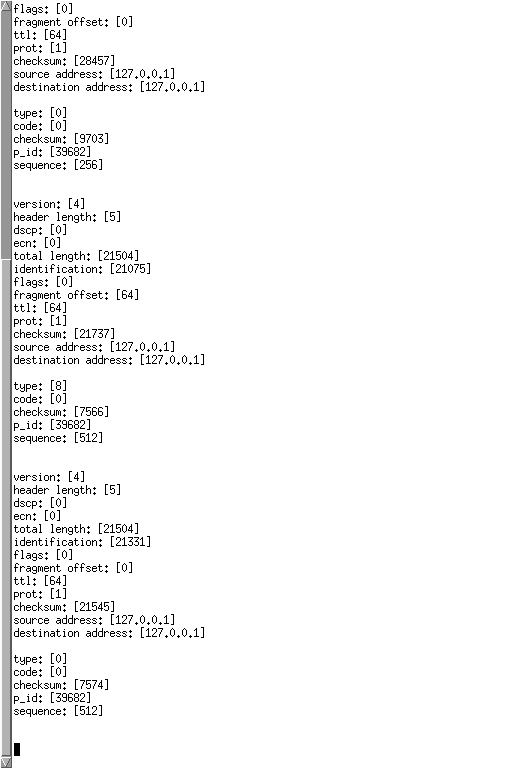
\includegraphics[width=\textwidth]{screenshots/deconstructed_headers.png}
  \caption{%
    Dissecting an \gls{icmp} ECHO REQUEST packet.
  }\label{echodissect}
\end{figure}

\begin{figure}[H]
  \centering
  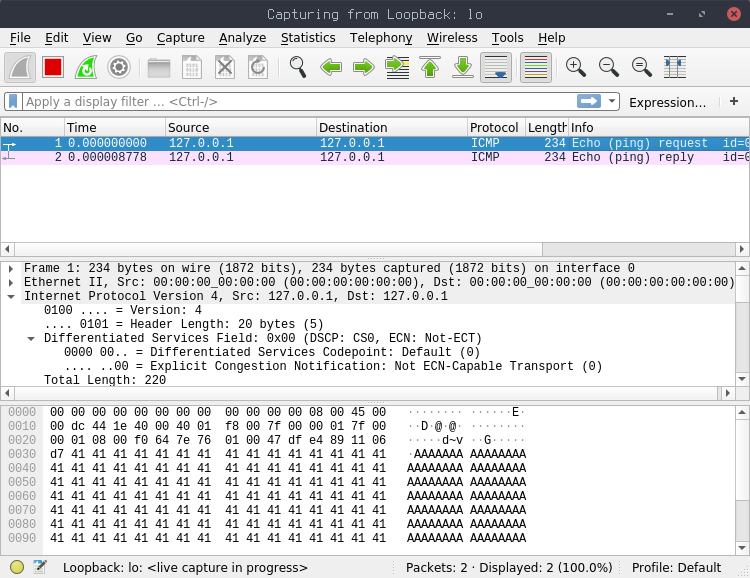
\includegraphics[width=\textwidth]{screenshots/ping_send_success.png}
  \caption{%
    Screenshot of wireshark showing a successful send of an \gls{icmp} ECHO REQUEST packet.
  }\label{pingsuccess}
\end{figure}

\begin{figure}[H]
  \centering
  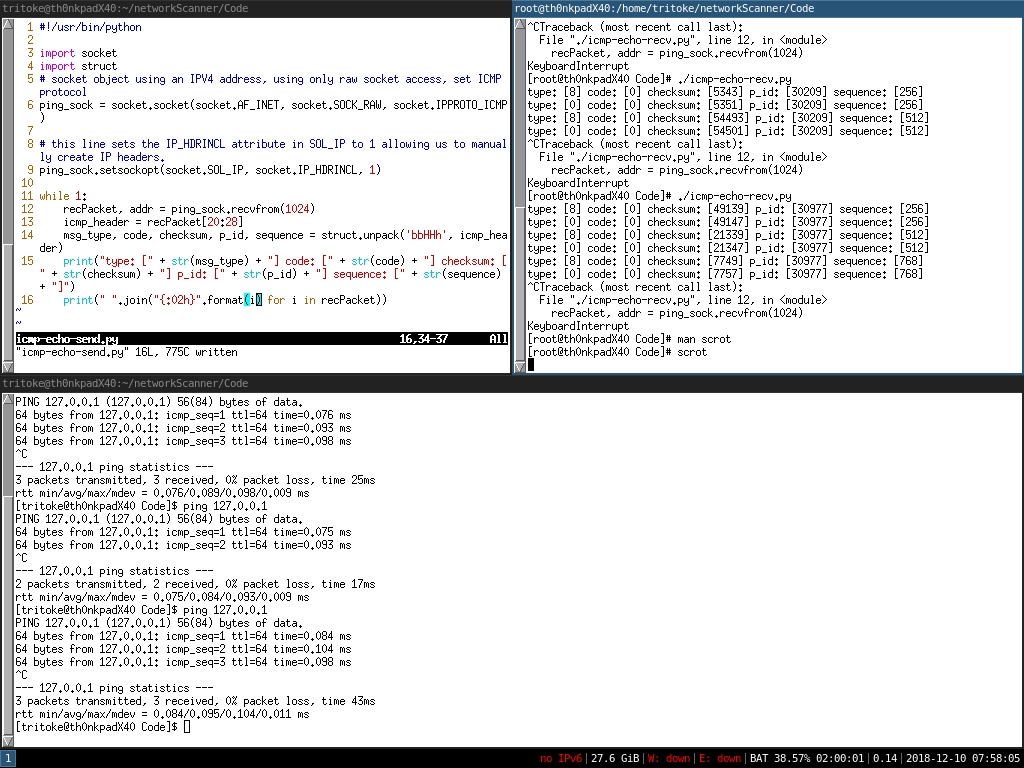
\includegraphics[width=\textwidth]{screenshots/local_self_ping.png}
  \caption{%
    Screenshot showing me first successfully dissecting an \gls{icmp} ECHO REQUEST packet.
  }\label{dissectsuccess}
\end{figure}

Having done these prototypes I have identified that it would probably be best to abstract the
code for dissecting all the headers i.e.\ \gls{icmp}, \gls{tcp} and \gls{ip} into classes
where I can just pass the received packet into the class and have it dissect it for me and then
I will also get access to some of the benefits of classes such as the \verb|__repr__| method
which is called when you print classes out and allows me to control what is printed out.
Before I started to write the final piece I wanted to make a prototype ping scanner, as this
would allow me to get a feel for making a scanner as well as further exploring low level protocol
interactions.

\begin{lstlisting}[label=pingscan,caption=An attempt at making a ping scanner.]
#!/usr/bin/python3.7
from os import getcwd, getpid
import sys
sys.path.append("../modules/")

import ip_utils

import socket
from functools import partial
from itertools import repeat
from multiprocessing import Pool
from contextlib import closing
from math import log10, floor
from typing import List, Tuple
import struct
import time


def round_significant_figures(x: float, n: int) -> float:
    """
    rounds x to n significant figures.
    round_significant_figures(1234, 2) = 1200.0
    """
    return round(x, n-(1+int(floor(log10(abs(x))))))


def recieved_ping_from_addresses(ID: int, timeout: float) -> List[Tuple[str, float, int]]:
    """
    Takes in a process id and a timeout and returns the list of addresses which sent
    ICMP ECHO REPLY packets with the packed id matching ID in the time given by timeout.
    """
    ping_sock = socket.socket(socket.AF_INET, socket.SOCK_RAW, socket.IPPROTO_ICMP)
    time_remaining = timeout
    addresses = []
    while True:
        time_waiting = ip_utils.wait_for_socket(ping_sock, time_remaining)
        if time_waiting == -1:
            break
        time_recieved = time.time()
        recPacket, addr = ping_sock.recvfrom(1024)
        ip_header = recPacket[:20]
        ip_hp_ip_v, ip_dscp_ip_ecn, ip_len, ip_id, ip_flgs_ip_off, ip_ttl, ip_p, ip_sum, ip_src, ip_dst = struct.unpack('!BBHHHBBHII', ip_header)
        icmp_header = recPacket[20:28]
        msg_type, code, checksum, p_id, sequence = struct.unpack('bbHHh', icmp_header)
        time_remaining -= time_waiting
        time_sent = struct.unpack("d", recPacket[28:28+struct.calcsize("d")])[0]
        time_taken = time_recieved - time_sent
        if p_id == ID:
            addresses.append((str(addr[0]), float(time_taken), int(ip_ttl)))
        elif time_remaining <= 0:
            break
        else:
            continue
    return addresses


with closing(socket.socket(socket.AF_INET, socket.SOCK_RAW, socket.IPPROTO_ICMP)) as ping_sock:
    addresses = ip_utils.ip_range("192.168.1.0/24")
    local_ip = ip_utils.get_local_ip()
    if addresses is not None:
        addresses_to_scan = filter(lambda x: x!=local_ip, addresses)
    else:
        print("error with ip range specification")
        exit()
    p = Pool(1)
    ID = getpid()&0xFFFF
    replied = p.apply_async(recieved_ping_from_addresses, (ID, 2))
    for address in zip(addresses_to_scan, repeat(1)):
        try:
            packet = ip_utils.make_icmp_packet(ID)
            ping_sock.sendto(packet, address)
        except PermissionError:
            pass
    p.close()
    p.join()
    hosts_up = replied.get()
    print("\n".join(map(lambda x: f"host: [{x[0]}]\tresponded to an ICMP ECHO REQUEST in {round_significant_figures(x[1], 2):<10} seconds, ttl: [{x[2]}]", hosts_up)))
\end{lstlisting}

\begin{figure}[H]
  \centering
  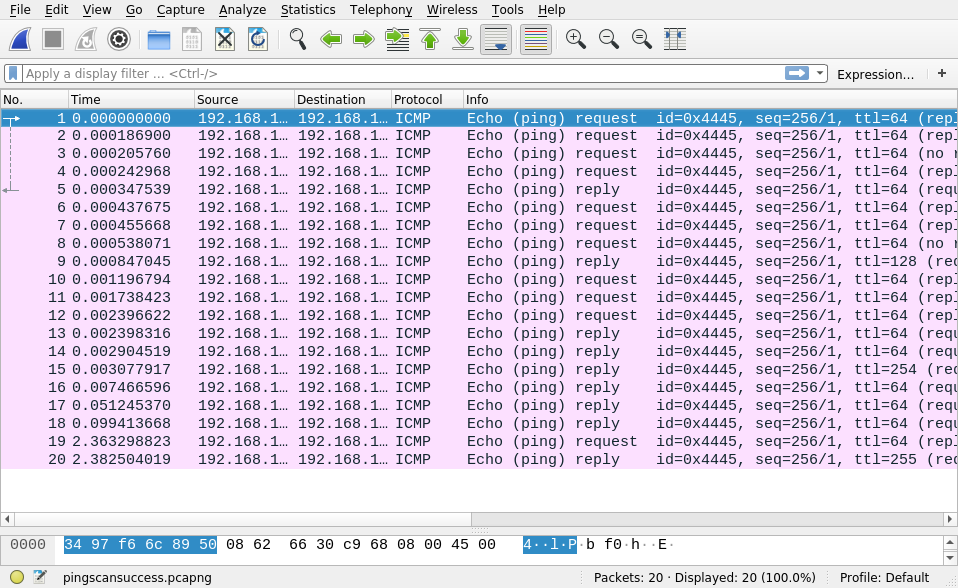
\includegraphics[width=\textwidth]{screenshots/pingscan.png}
  \caption{%
    Screenshot of wireshark showing a successful ping scan.
  }\label{pingscansuccess}
\end{figure}

\lstset{language=C}
\begin{lstlisting}[label=pingscanout,caption=The output of from the ping scanner on the run which generated the \gls{pcap} file in figure~\ref{pingscansuccess}]
$ sudo ./ping_scan.py
host: [192.168.1.1]	responded to an ICMP ECHO REQUEST in 0.00037    seconds, ttl: [64]
host: [192.168.1.35] responded to an ICMP ECHO REQUEST in 0.00042    seconds, ttl: [128]
host: [192.168.1.37] responded to an ICMP ECHO REQUEST in 0.002      seconds, ttl: [64]
host: [192.168.1.117] responded to an ICMP ECHO REQUEST in 0.0017     seconds, ttl: [64]
host: [192.168.1.176] responded to an ICMP ECHO REQUEST in 0.0014     seconds, ttl: [254]
host: [192.168.1.14] responded to an ICMP ECHO REQUEST in 0.0072     seconds, ttl: [64]
host: [192.168.1.246] responded to an ICMP ECHO REQUEST in 0.049      seconds, ttl: [64]
host: [192.168.1.8] responded to an ICMP ECHO REQUEST in 0.099      seconds, ttl: [64]
\end{lstlisting}

Now that I have done these prototypes I am fairly certain about how I will structure the rest of
my scanners, how to interact with Python's socket programming interface and how I can use the
struct module to make and dissect packets. My general plan for the scanners will be to start
a process that listens for responses for a set amount of time and then start sending the packets
in a different process before waiting for the listening process to get all the responses back and
collecting the results from that process.

\subsection{Acceptable Limitations}

Originally I had planned to include dedicated operating system detection as an option
however I ran out of time having implemented version detection. However it still does
Operating system detection partially as some \glspl{service} are linux only and while doing
\gls{service} and version detection especially the \gls{cpe} parts
of the matched \gls{service}/version will contain operating system information, such as
microsoft ActiveSync would indicate that the system being scanned was a windows system
which is reflected in the match directive and attached CPE information:
\begin{verbatim}
match activesync m|^.\0\x01\0[^\0]\0[^\0]\0[^\0]\0[^\0]\0[^\0]\0.*
\0\0\0$|s p/Microsoft ActiveSync/ o/Windows/ cpe:/a:microsoft:acti
vesync/ cpe:/o:microsoft:windows/a
\end{verbatim}

\subsection{Test Strategy}

I am going to use two different methods to test my program:
\begin{enumerate}
\item{Unit testing}
\item{Wireshark}
\end{enumerate}
I am using two separate testing strategies because they are both good at different things,
both of which I need to show that my project works. Firstly I am using unit testing to test
some general purpose functions which are pure functions (are independent of the current state
of the machine) such as \verb|ip_range()| and other functions which I can just check the returned
value against what it should be.

Wireshark is useful for the other half of the program which uses impure functions and the low level 
networking e.g.\ \verb|make_tcp_packet()|. Wireshark makes this easy by allowing capture of all the 
\glspl{pkt} going over the wire, as well as this it has a vast array of \gls{pkt} decoders (2231 in 
my install) which it can use to dissect almost any \gls{pkt} that would be on the network. The main 
benefit of wireshark is that I can see my scanners sending \glspl{pkt} and then check whether the 
parsers that I have written for the different protocols are working. I can also check that the 
\glspl{csum} in each of the various protocols is valid as wireshark does \gls{csum} verification for 
various protocols. 

\section{Design}

\subsection{Overall System Design (High Level Overview)}

There are two types of scanning implemented for different scan types in my program.
\begin{itemize}
  \item{\verb|Connect()|}
  \item{version}
  \item{listener / sender}
\end{itemize}
\verb|Connect()| scanning is the simplest in that it takes in a list of \glspl{port} and simply 
calls the \verb|socket.connect()| method on it and sees whether it can connect or not and the 
\glspl{port} are marked accordingly as open or closed. 

Version scanning is very similar to \verb|Connect()| scanning in that it takes in a list of 
\glspl{port} and connects to them, except it then sends a probe to the target to elicit a response 
and gain some information about the \gls{service} running behind the \gls{port}.

Listener / sender scanning does exactly what it says on the tin: it sets up a ``listener'' in 
another process to listen for responses from the host which the ``sender'' is sending \glspl{pkt} 
to. It can then differentiate between open, open|filtered, filtered and closed \glspl{port} based on 
whether it receives a \gls{pkt} back and what flags (part of\gls{tcp} \glspl{pkt} are a one byte 
long section which store ``flags'' where each bit in the byte represents a different flag) are set 
in the received \gls{pkt}. 

\subsection{Design of User Interfaces HCI}

I have designed my system to have a similar interface to the most common tool currently used: nmap 
this is because I believe that having a familiar interface will not only make it easier for someone 
who is familiar with nmap to use my tool it also makes it so that anything learnt using either tool 
is applicable to both which benefits everyone.

Based on this perception I have used the same option flags as nmap as well as similar help messages 
and an identical call signature (how the program is used on the command line). Running 
\verb|./netscan.py <options> <target_spec>| is identical to \verb|nmap <options> <target_spec>| in 
terms of which scan types will be run, which hosts will be scanned and which \glspl{port} are 
scanned. Below you can see the help message generated by \verb|./netscan.py --help|.

\begin{verbatim}
usage: netscan.py [-h] [-Pn] [-sL] [-sn] [-sS] [-sT] [-sU] [-sV] [-p PORTS]
                  [--exclude_ports EXCLUDE_PORTS]
                  target_spec

positional arguments:
  target_spec           specify what to scan, i.e. 192.168.1.0/24

optional arguments:
  -h, --help            show this help message and exit
  -Pn                   assume hosts are up
  -sL                   list targets
  -sn                   disable port scanning
  -sS                   TCP SYN scan
  -sT                   TCP connect scan
  -sU                   UDP scan
  -sV                   version scan
  -p PORTS, --ports PORTS
                        scan specified ports
  --exclude_ports EXCLUDE_PORTS
                        ports to exclude from the scan
\end{verbatim}

It shows clearly which are required arguments and which are optional ones, as well as what
each argument actually does. It also allows some some arguments to be called with either
a short format e.g.\ \verb|-p| and with a most verbose format \verb|--ports| this allows
the user to be clearer if they are using the tool as part of an automated script to perform
scanning as it is more immediately obvious what the more verbose flags do.

\subsection{System Algorithms}

\begin{figure}[H]
  \centering
  \begin{framed}
    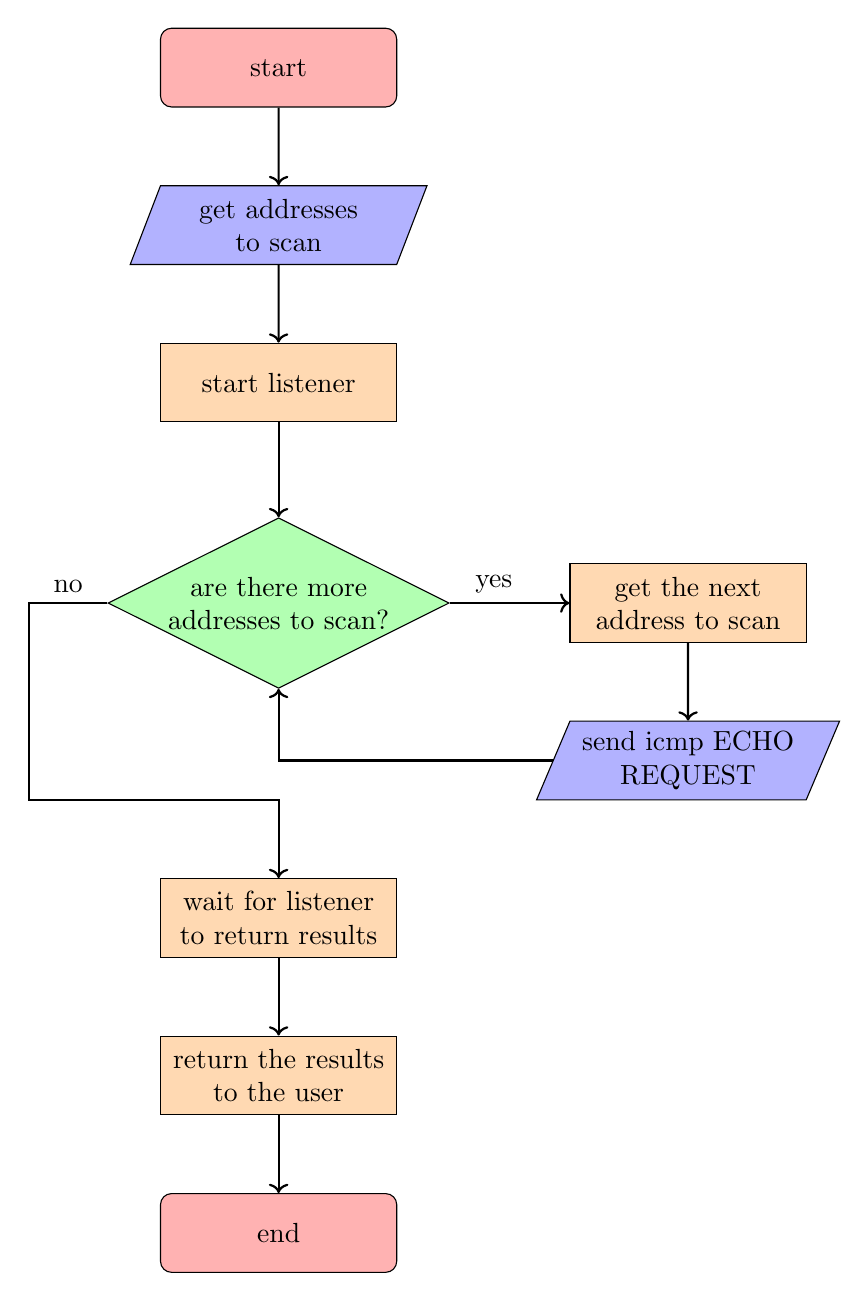
\begin{tikzpicture}[node distance=2cm]
      \node [startstop] (start) {start};
      \node [io, below of=start, text width=3cm] (input) {get addresses to scan};
      \node [process, below of=input] (listener) {start listener};
      \node [decision, below of=listener, text width=3cm, yshift=-0.8cm] (loop) {are there more addresses to scan?};
      \node [process, right of=loop, xshift=3.2cm] (get) {get the next address to scan};
      \node [io, below of=get, text width=3cm] (send) {send \gls{icmp} ECHO REQUEST};
      \node [process, below of=loop, yshift=-2cm] (wait) {wait for listener to return results};
      \node [process, below of=wait] (output) {return the results to the user};
      \node [startstop, below of=output] (end) {end};

      \draw [arrow] (start) -- (input);
      \draw [arrow] (input) -- (listener);
      \draw [arrow] (listener) -- (loop);
      \draw [arrow] (loop) -- node[midway,above,xshift=-0.2cm] {yes} (get);
      \draw [arrow] (get) -- (send);
      \draw [arrow] (send) -| node[midway,above,xshift=2cm] {} (loop);
      \draw [arrow] (loop) -- ([xshift=-1cm]loop.west) node[above,xshift=0.5cm] {no} -- ([xshift=-1cm,yshift=-2.5cm]loop.west) -| (wait);
      \draw [arrow] (wait) -- (output);
      \draw [arrow] (output) -- (end);

    \end{tikzpicture}
  \end{framed}
  \caption{%
    The logic for how I will do Ping Scanning.
  }\label{pingscanflow}
\end{figure}

\begin{figure}[H]
  \centering
  \begin{framed}
    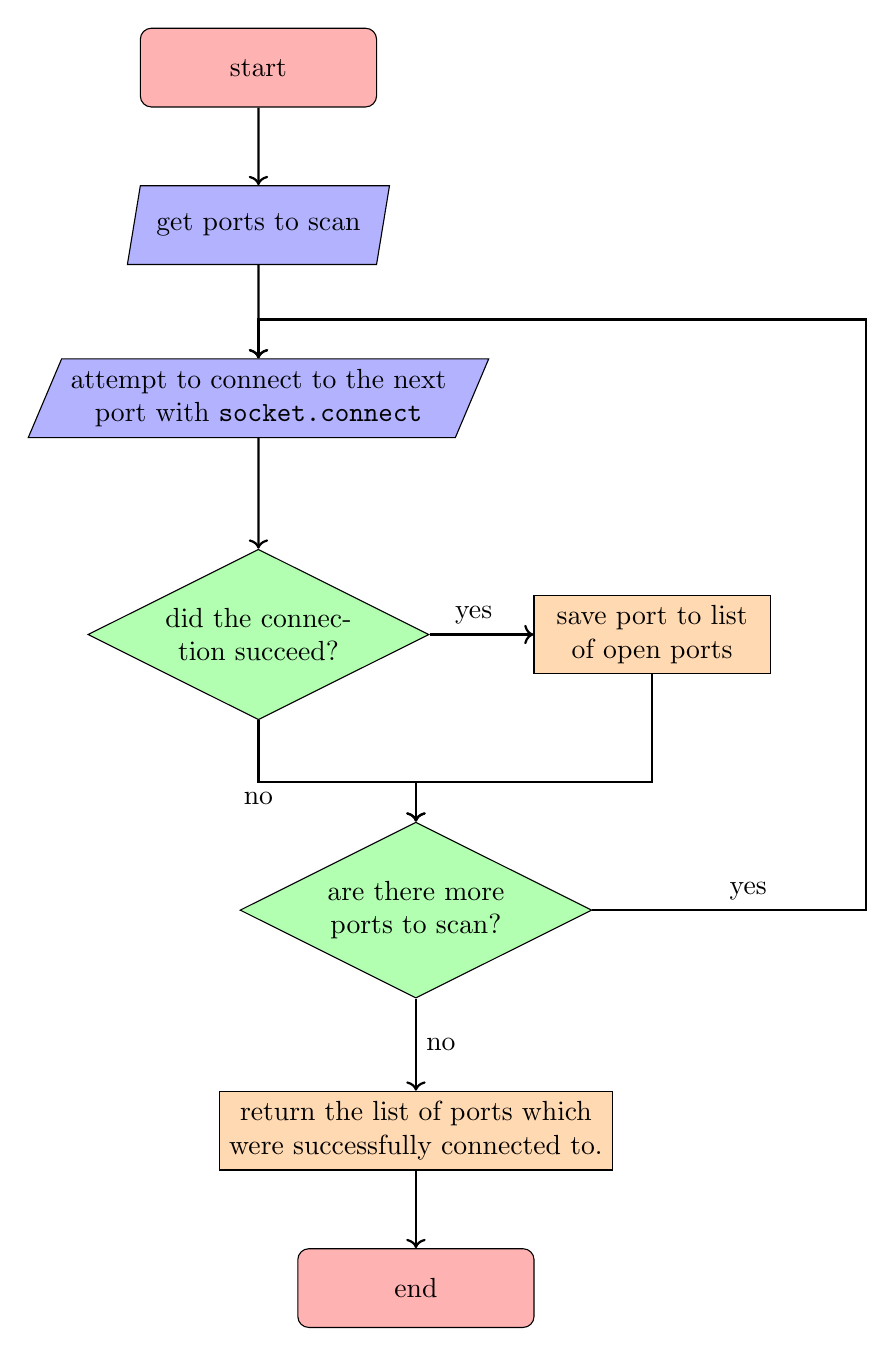
\begin{tikzpicture}[node distance=2cm]
      \node [startstop] (start) {start};
      \node [io, below of=start] (get) {get ports to scan};
      \node [io, below of=get, text width = 5cm,yshift=-0.2cm] (connect) {attempt to connect to the next port with \verb|socket.connect|};
      \node [decision, below of=connect, text width=3cm, yshift=-1cm] (save) {did the connection succeed?};
      \node [process, right of=save, xshift=3cm] (add) {save port to list of open ports};
      \node [decision, below of=save, text width=3cm, yshift=-1.5cm, xshift=2cm] (loop) {are there more ports to scan?};
      \node [process, below of=loop, yshift=-0.8cm, text width=5cm] (return) {return the list of ports which were successfully connected to.};
      \node [startstop, below of=return] (end) {end};

      \draw [arrow] (start) -- (get);
      \draw [arrow] (get) -- (connect);
      \draw [arrow] (connect) -- (save);
      \draw [arrow] (save) -- node[midway,above,xshift=-0.1cm] {yes} (add);
      \draw [arrow] (save) |- node[midway, below] {no} ([yshift=0.5cm]loop.north) -- (loop);
      \draw [arrow] (add) |- ([yshift=0.5cm]loop.north) -- (loop);
      \draw [arrow] (loop) -| node[midway, above, xshift=-1.5cm] {yes} ([xshift=5cm,yshift=1cm]connect.east) -| (connect.north);
      \draw [arrow] (loop) -- node[midway, right] {no} (return);
      \draw [arrow] (return) -- (end);

    \end{tikzpicture}
  \end{framed}
  \caption{%
    The logic for how I will do TCP connect Scanning.
  }\label{tcpconnectscanflow}
\end{figure}

\begin{figure}[H]
  \centering
  \begin{framed}
    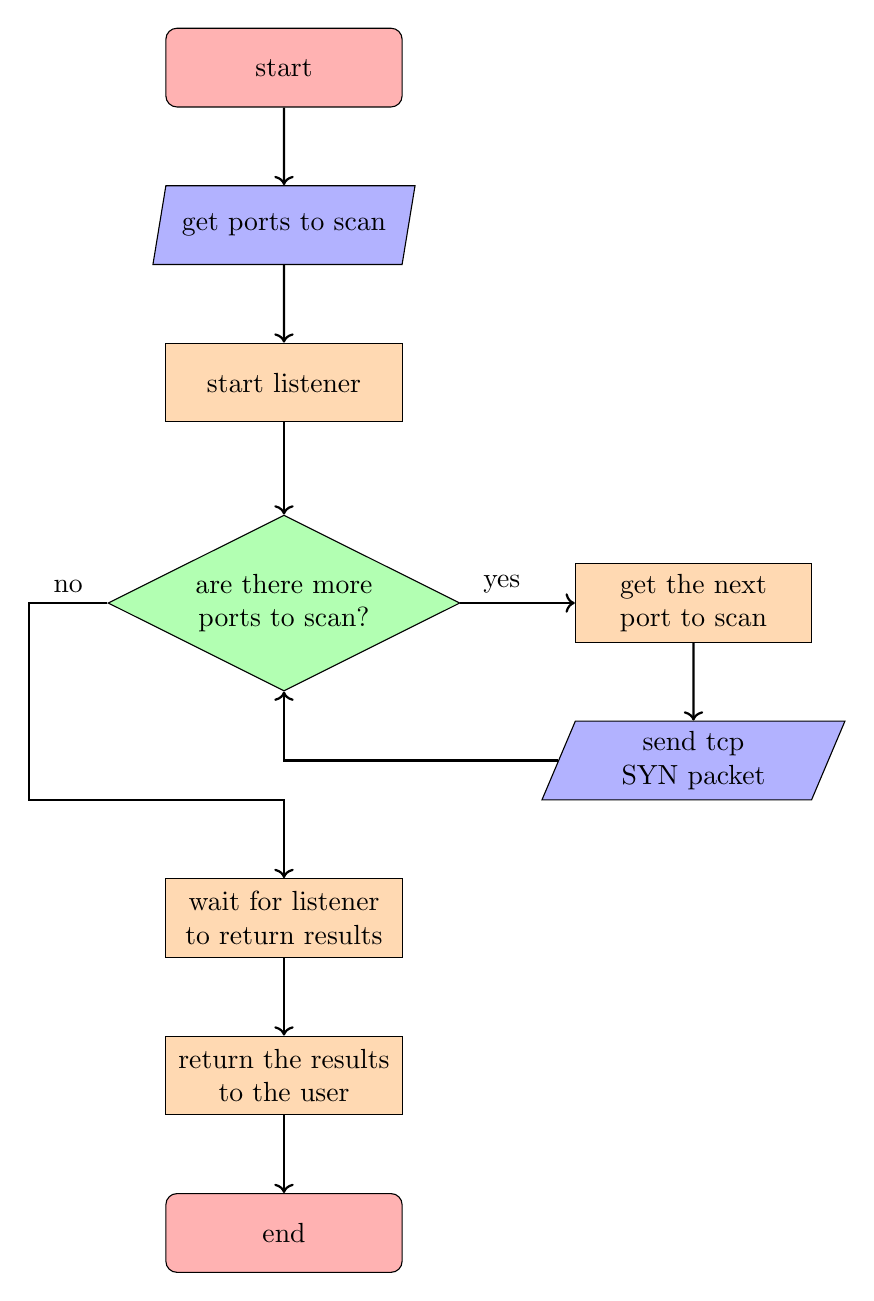
\begin{tikzpicture}[node distance=2cm]
      \node [startstop] (start) {start};
      \node [io, below of=start, text width=3cm] (input) {get ports to scan};
      \node [process, below of=input] (listener) {start listener};
      \node [decision, below of=listener, text width=3cm, yshift=-0.8cm] (loop) {are there more ports to scan?};
      \node [process, right of=loop, xshift=3.2cm] (get) {get the next port to scan};
      \node [io, below of=get, text width=3cm] (send) {send \gls{tcp} SYN packet};
      \node [process, below of=loop, yshift=-2cm] (wait) {wait for listener to return results};
      \node [process, below of=wait] (output) {return the results to the user};
      \node [startstop, below of=output] (end) {end};

      \draw [arrow] (start) -- (input);
      \draw [arrow] (input) -- (listener);
      \draw [arrow] (listener) -- (loop);
      \draw [arrow] (loop) -- node[midway,above,xshift=-0.2cm] {yes} (get);
      \draw [arrow] (get) -- (send);
      \draw [arrow] (send) -| node[midway,above,xshift=2cm] {} (loop);
      \draw [arrow] (loop) -- ([xshift=-1cm]loop.west) node[above,xshift=0.5cm] {no} -- ([xshift=-1cm,yshift=-2.5cm]loop.west) -| (wait);
      \draw [arrow] (wait) -- (output);
      \draw [arrow] (output) -- (end);

    \end{tikzpicture}
  \end{framed}
  \caption{%
    The logic for how I will do TCP SYN scanning.
  }\label{tcpsynscanflow}
\end{figure}

\begin{figure}[H]
  \centering
  \begin{framed}
    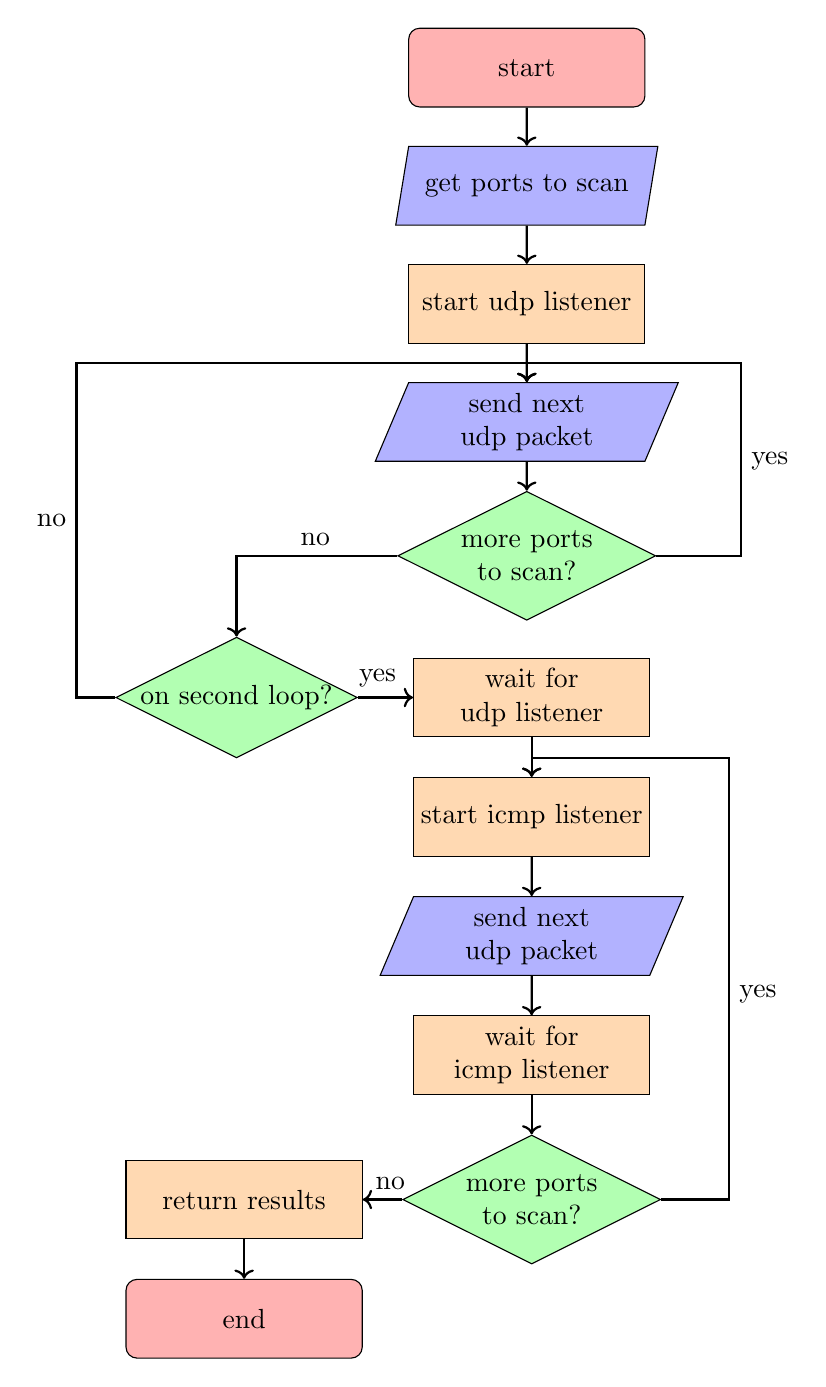
\begin{tikzpicture}[node distance=1.5cm]
      \node [startstop] (start) {start};
      \node [io,below of=start] (get) {get ports to scan};
      \node [process, below of=get] (udp listener) {start udp listener};
      \node [io, below of=udp listener, inner sep=0] (send 1) {send next \gls{udp} packet};
      \node [decision, below of=send 1, text width=2cm, yshift=-0.2cm] (loop 1) {more ports to scan?};
      \node [decision, below of=loop 1, left=0.5cm of loop 1, yshift=-0.3cm] (loop 2) {on second loop?};
      \node [process, right=0.7cm of loop 2] (udp wait) {wait for \gls{udp} listener};
      \node [process, below=0.5cm of udp wait] (icmp listener) {start \gls{icmp} listener};
      \node [io, below=0.5cm of icmp listener, inner sep=0] (send 2) {send next \gls{udp} packet};
      \node [process, below=0.5cm of send 2] (icmp wait) {wait for \gls{icmp} listener};
      \node [decision, below=0.5cm of icmp wait, text width = 2cm] (loop 3) {more ports to scan?};
      \node [process, left=0.5cm of loop 3] (return) {return results};
      \node [startstop, below=0.5cm of return] (end) {end};

      \draw [arrow] (start) -- (get);
      \draw [arrow] (get) -- (udp listener);
      \draw [arrow] (udp listener) -- (send 1);
      \draw [arrow] (send 1) -- (loop 1);
      \draw [arrow] (loop 1.east) -| ([xshift=1cm,yshift=0.75cm]send 1.east) node [right,yshift=-1.25cm] {yes} -| (send 1.north);
      \draw [arrow] (loop 1) -| node [above, xshift=1cm] {no} (loop 2);
      \draw [arrow] (loop 2.west) -| ([xshift=-4cm,yshift=0.75cm]send 1.west) node [left,yshift=-2cm] {no} -| (send 1.north);
      \draw [arrow] (loop 2) -- node [xshift=-0.1cm,above] {yes} (udp wait);
      \draw [arrow] (udp wait) -- (icmp listener);
      \draw [arrow] (icmp listener) -- (send 2);
      \draw [arrow] (send 2) -- (icmp wait);
      \draw [arrow] (icmp wait) -- (loop 3);
      \draw [arrow] (loop 3.east) -| ([xshift=1cm,yshift=0.75cm]icmp listener.east) node [right,yshift=-3cm] {yes} -| (icmp listener);
      \draw [arrow] (loop 3) -- node [above,xshift=0.1cm] {no} (return);
      \draw [arrow] (return) -- (end);

    \end{tikzpicture}
  \end{framed}
  \caption{%
    The logic behind how \gls{udp} scanning works.
  }\label{udpscanflow}
\end{figure}


\begin{figure}[H]
  \centering
  \begin{framed}
    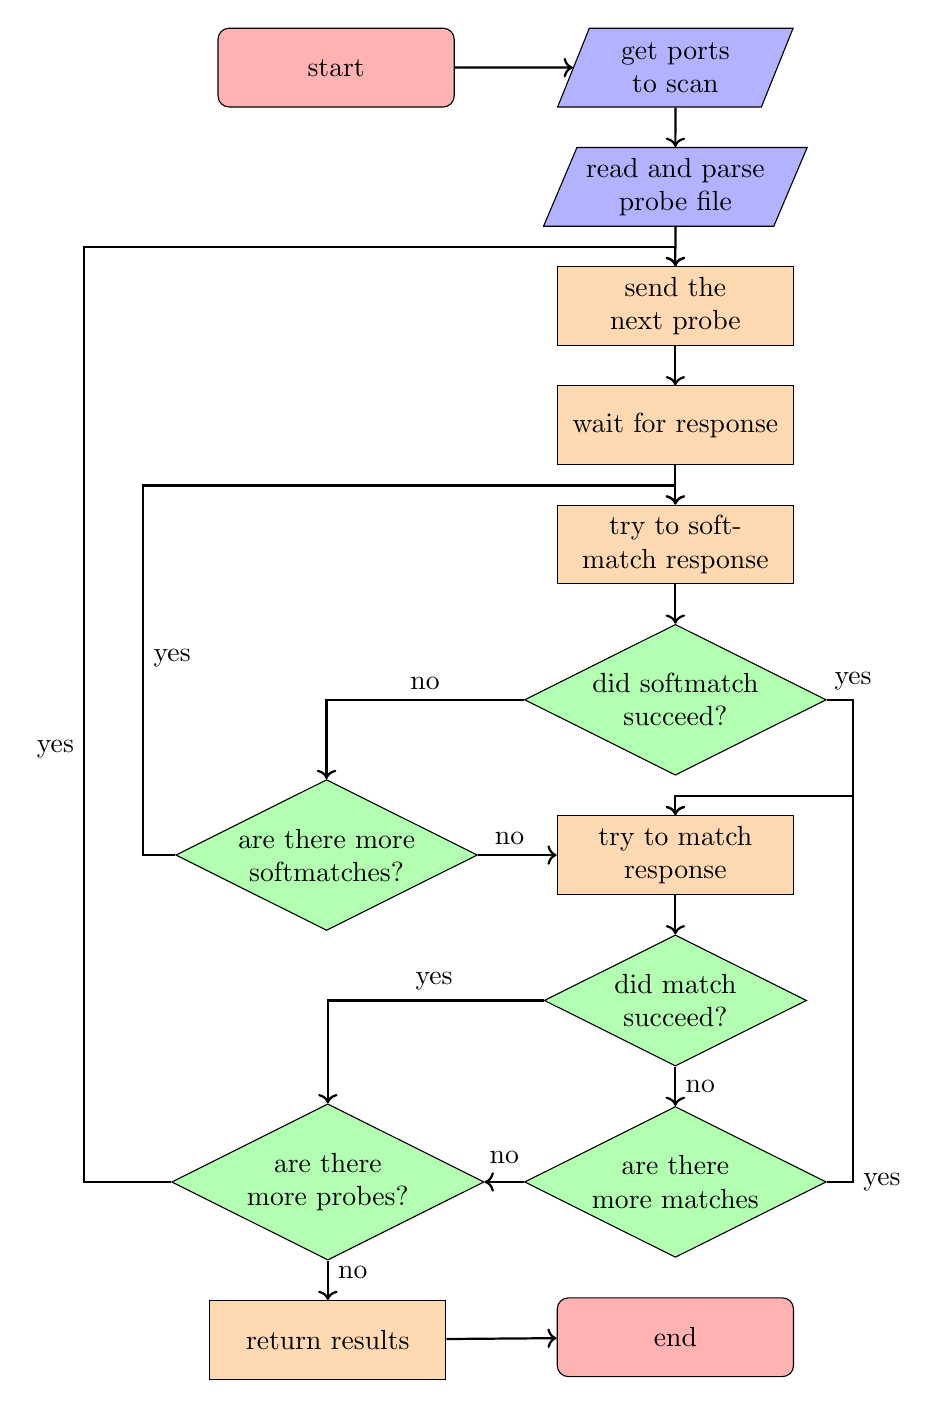
\begin{tikzpicture}[node distance=1.5cm]
      \node [startstop] (start) {start};
      \node [io, right=1.5cm of start, text width=2cm] (get ports) {get ports to scan};
      \node [io, below=0.5cm of get ports, text width=2.5cm] (parse probes) {read and parse probe file};
      \node [process, below=0.5cm of parse probes] (send probe) {send the next probe};
      \node [process, below=0.5cm of send probe] (wait) {wait for response};
      \node [process, below=0.5cm of wait] (softmatch) {try to softmatch response};
      \node [decision, below=0.5cm of softmatch, text width=2.5cm] (softmatched) {did softmatch succeed?};
      \node [process, below=0.5cm of softmatched] (match) {try to match response};
      \node [decision, left=1cm of match, text width=2.5cm] (softmatch loop) {are there more softmatches?};
      \node [decision, below=0.5cm of match, text width=2cm] (matched) {did match succeed?};
      \node [decision, below=0.5cm of matched, text width=2.5cm] (match loop) {are there more matches};
      \node [decision, left=0.5cm of match loop, text width=2.5cm] (probe loop) {are there more probes?};
      \node [process, below=0.5cm of probe loop] (return) {return results};
      \node [startstop, below=0.5cm of match loop] (end) {end};

      \draw [arrow] (start) -- (get ports);
      \draw [arrow] (get ports) -- (parse probes);
      \draw [arrow] (parse probes) -- (send probe);
      \draw [arrow] (send probe) -- (wait);
      \draw [arrow] (wait) -- (softmatch);
      \draw [arrow] (softmatch) -- (softmatched);
      \draw [arrow] (softmatched.east) -| node[above] {yes} ([yshift=0.75cm,xshift=0.75cm]match.east) -| (match);
      \draw [arrow] (softmatched) -| node[above, xshift=1.25cm] {no} (softmatch loop);
      \draw [arrow] (softmatch loop) -- node [above, xshift=-0.1cm] {no} (match);
      \draw [arrow] (softmatch loop)-|node[right,yshift=2.5cm]{yes}([xshift=-5.25cm,yshift=0.75cm]softmatch.west)-|(softmatch);
      \draw [arrow] (match) -- (matched);
      \draw [arrow] (match loop) -| node [right,] {yes} ([xshift=0.75cm,yshift=0.75cm] match.east) -| (match.north);
      \draw [arrow] (matched) -- node [right] {no} (match loop);
      \draw [arrow] (match loop) -- node [above, yshift=0.1cm] {no} (probe loop);
      \draw [arrow] (matched) -| node [above, xshift=1.35cm] {yes} (probe loop);
      \draw [arrow] (probe loop) -| node [left,yshift=5.5cm] {yes} ([xshift=-6cm,yshift=0.75cm]send probe.west) -| (send probe);
      \draw [arrow] (probe loop) -- node [midway, right, yshift=0.1cm] {no} (return);
      \draw [arrow] (return) -- (end);

    \end{tikzpicture}
  \end{framed}
  \caption{%
    The logic behind how version detection works.
  }\label{versiondetectflow}
\end{figure}


\subsection{Input data Validation}

My program takes very little input from the user which means that there is a very low chance of the 
program crashing due to user input error as the errors are detected All data which is entered is 
either parsed using a regular expression with the case of the \glspl{port} directive (\verb|-p|) or 
is run through checking functions like \verb|ip_utils.is_valid_ip|. As well as using these checking 
functions whenever an~\gls{ipaddr} is converted between ``long form'' and ``dot form'' which is used 
in every type of scanning.

\subsection{Proposed Algorithms for complex structures (flow charts or Pseudo Code)}

\begin{algorithm}
  \caption{%
  My algorithm for turning a \gls{cidr} specified \gls{subnet} into a list of actual \gls{ipaddr}es
}\label{ip_range}
  \begin{algorithmic}[1]
    \Procedure{ip\_range}{}
    \State{$\textit{network\_bits} \gets \text{number of network bits specified}$}
    \State{$\textit{ip} \gets \text{base IP address}$}
    \State{$\textit{mask} \gets 0$}
    \For{$\textit{maskbit} \gets (32-\textit{network\_bits}),31$}
      \State{$\textit{mask} \gets \textit{mask} + 2^\textit{maskbit}$}
    \EndFor{}
    \State{$\textit{lower\_bound} \gets \text{\textit{ip} AND \textit{mask}}$}
    \Comment{zero the last 32-\textit{network\_bits}}
    \State{$\textit{upper\_bound} \gets \text{\textit{ip} OR (\textit{mask} XOR 0xFFFFFFFF)}$}
    \Comment{turn the last 32-\textit{network\_bits} to ones}
    \State{$\textit{addresses} \gets \text{empty list}$}
    \For{$\textit{address} \gets \textit{lower\_bound},\textit{upper\_bound}$}
      \State{append \Call{convert\_to\_dot}{\textit{address}} to \textit{addresses}}
    \EndFor{}
    \Return{\textit{addresses}}
    \EndProcedure{}
  \end{algorithmic}
\end{algorithm}

\begin{algorithm}
  \caption{%
    My algorithm for pretty-printing a dictionary of lists of\gls{port}numbers
    such that ranges are specified as start-end instead of start,start+1,\ldots,end
  }\label{collapse}
  \begin{algorithmic}[1]
  \Procedure{collapse}{}
    \State{$\textit{port\_dictionary} \gets \text{dictionary of lists of\gls{port}numbers}$}
    \State{$\textit{key\_results} \gets \text{empty list}$}
    \Comment{stores the formatted result for each key}
    \For{\textit{key} in \textit{port\_dictionary}}
      \State{$\textit{ports} \gets \text{\textit{port\_dict}[\textit{key}]}$}
      \State{$\textit{result} \gets \textit{key} + \text{``:\{''}$}
      \If{\textit{ports} is empty}
        \State{$\textit{new\_sequence} \gets FALSE$}
        \For{$\textit{index} \gets 1,\text{(length of \textit{ports})}-1$}
          \State{$\textit{port} = \text{\textit{ports}[\textit{index}]}$}
          \If{$\textit{index} = 0$}
            \State{$\textit{result} \gets \textit{result} + \textit{ports}[0]$}
            \Comment{append the first element}
            \If{$\text{\textit{ports}[\textit{index}+1]} = \textit{port} + 1$}
              \State{$\textit{result} \gets \textit{result}+\text{``-''}$}
              \Comment{begin a new sequence}
            \Else{}
              \State{$\textit{result} \gets \textit{result} + \text{``,''}$}
              \Comment{not a sequence}
            \EndIf{}
          \ElsIf{$\textit{port} + 1 \not= \text{\textit{ports}[\textit{index}+1]}$}
          \Comment{break in sequence}
            \State{$\textit{result} \gets \textit{result} + \textit{port} + \text{``,''}$}
            \State{$\textit{new\_sequence} \gets \textit{TRUE}$}
          \ElsIf{$\textit{port}+1 = \text{\textit{ports}[\textit{index}+1]} \And \textit{new\_sequence}$}
            \State{$\textit{result} \gets \textit{result} + \text{``-''}$}
            \State{$\textit{new\_sequence} \gets \textit{FALSE}$}
          \EndIf{}
        \EndFor{}
      \State{$\textit{result} \gets \textit{result} + \text{\textit{ports}[(length of \textit{ports})-1]} + \text{``\}''}$}
      \State{append \textit{result} to \textit{key\_results}}
      \EndIf{}
    \EndFor{}
    \Return{``\{'' + (\textit{key\_results} separated by ``, '') + ``\}''}
  \EndProcedure{}
  \end{algorithmic}
\end{algorithm}

\section{Technical Solution}

\subsection{Overview to direct the examiner to areas of complexity and explain design evidence}

\section{Testing}

\subsection{Test Plan}

\subsection{Test Table / Testing Evidence (Core: lots of screenshots)}

\section{Evaluation}

\subsection{Reflection on final outcome}

\subsection{Evaluation against objectives, end user feedback}

\subsection{Potential improvements}

\section{Appendices}
\lstset{language=python}

\subsection{icmp\_ping}
\lstinputlisting[caption=A prototype program for sending ICMP ECHO REQEST packets,label=icmpechosend]{../../Code/icmp_ping/icmp_echo_send.py}
\lstinputlisting[caption=A prototype program for receiving ICMP ECHO REQEST packets,label=icmpechorecv]{../../Code/icmp_ping/icmp_echo_recv.py}

\subsection{ping\_scanner}
\lstinputlisting[caption=A prototype program for performing `ping' scans,label=pingscanner]{../../Code/ping_scanner/ping_scan.py}

\subsection{subnet\_to\_addresses}
\lstinputlisting[caption=A program which translates a CIDR specified subnet into a list of addresses and prints them out in sorted order,label=subnettoaddresses]{../../Code/subnet_to_address.py}

\subsection{tcp\_scan}
\verb|Connect()| scanning
\lstinputlisting[caption=prototype TCP Connect() scanner only attempting to detect the state of port 22,label=connectsshattempt]{../../Code/tcp_scan/connect_scan/ssh_attempt.py}
\lstinputlisting[caption=A program that performs TCP Connect() scanning, label=connectscanportlist]{../../Code/tcp_scan/connect_scan/scan_port_list.py}

SYN scanning
\lstinputlisting[caption=A prototype program that tries to detect the state of port 22 via TCP SYN scanning (aka half open scanning),label=synsshattempt]{../../Code/tcp_scan/syn_scan/ssh_attempt.py}
\lstinputlisting[caption=A program that performs TCP SYN scanning (aka half open scanning),label=synscanportlist]{../../Code/tcp_scan/syn_scan/scan_port_list.py}

\subsection{udp\_scan}
\lstinputlisting[caption=A prototype program to detect whether UDP port 53 is open on a target machine, label=dnsattempt]{../../Code/udp_scan/dns_attempt.py}
\lstinputlisting[caption=A program for performing scans on UDP ports.,label=udpscanportlist]{../../Code/udp_scan/scan_port_list.py}
\lstinputlisting[caption=A program I made to open a port via UDP for testing my UDP scanner.,label=openxport]{../../Code/udp_scan/open_X_port_to_UDP.py}

\subsection{version\_detection}
\lstinputlisting[caption=A program which does version detection on services.,label=versiondetection]{../../Code/version_detection/version_detection.py}

\subsection{modules}
\lstinputlisting[caption=A python module I wrote for parsing and holding the version detection probes from the nmap\_service\_probes file.,label=directives]{../../Code/modules/directives.py}
\lstinputlisting[caption=A python module I made to dissect and hold protocol headers.,label=headers]{../../Code/modules/headers.py}
\lstinputlisting[caption=A python module I wrote to contain lots of useful functions which I found I was declaring in multiple places and makign changes so I decided to keep an up to date central one.,label=iputils]{../../Code/modules/ip_utils.py}
\lstinputlisting[caption=A python module I made to hold all of the listeners I had made for each of the different scanning types.,label=listeners]{../../Code/modules/listeners.py}
\lstinputlisting[caption=A python module I made to hold all of the scanners I had made for each of the different scanning types.,label=scanners]{../../Code/modules/scanners.py}

\subsection{examples}
\lstinputlisting[caption=A program I wrote to run all of the example scripts I made from one main script to solve the issue of the PATH being used for determining import when I could use Pythons built in module structure instead.,label=runexamples]{../../Code/run_examples.py}

\subsection{netscan}
\lstinputlisting[caption=The program which provides the command line user interface for my projects functionality.,label=netscan]{../../Code/netscan.py}

\subsection{tests}
\lstinputlisting[caption=A few unit tests I wrote to cover some basic functions that I use as underpinnings for a lot of my other work so I wanted to make sure I hadn't accidentally broken any of them.,label=tests]{../../Code/tests/test_ip_utils.py}


\clearpage
\printnoidxglossaries{}

\end{document}
